\chapter{Evaluation}
\label{chap:evaluation}

\section{Evaluation Aspects}
\label{sec:evaluation-aspects}
    In this chapter, we evaluate the multi-bit spike train model on various aspects: 
    \begin{itemize}
        \item \textbf{Accuracy}: We compare the convergence speed and final accuracy of the multi-bit spike train model with the traditional 1-bit spike train model on various tasks and datasets.
        \item \textbf{Firing Rate}: We investigate how the increase of the bit width of the spike train affects the firing rate of the neurons in the network.
        \item \textbf{Quantizability}: We evaluate the accuracy of the multi-bit spike train model when quantized to lower precision.
        \item \textbf{Energy Consumption}: We evaluate the energy consumption of the multi-bit spike train model in practical scenarios.
        \item \textbf{Performance}: We present the performance data of the multi-bit spike train model on GPUs. 
    \end{itemize}

\section{Experimental Setup}
\label{sec:experimental-setup}
    We implement the multi-bit spike train model with SpikingJelly \cite{doi:10.1126/sciadv.adi1480} (version 0.0.0.0.15) using its PyTorch \cite{NEURIPS2019_9015} (version 2.5.0) backend. All experiments are conducted in the NVIDIA PyTorch container (nvcr.io/nvidia/pytorch:24.08-py3) on an NVIDIA GH200 super chip unless otherwise stated. 

    The multi-bit spike train model and the traditional 1-bit spike train model are tested on various tasks and datasets. The regular static datasets are imported from Torchvision \cite{10.1145/1873951.1874254} while the neuromorphic datasets are imported from Tonic \cite{lenz_2021_5079802}. 

    We measure the training accuracy (per batch), test accuracy (per epoch) and firing rate at certain points in the networks of the 1-bit to 8-bit spike train models. We then investigate the convergence, accuracy, firing rate, and quantizability of the multi-bit spike train model. 

    We mainly use the Fashion MNIST dataset \cite{xiao2017/online} and a convolutional neural network (CNN) \cite{726791} to set up the experiments of an image classification task. We will also show the results also hold on more complex datasets like CIFAR-10 \cite{Krizhevsky2009}. 

    In the following sections, the input images from Fashion MNIST are converted to spike trains using the Poisson encoding method. The CNN has a structure of $28\times 28 - 8c5 - 2a - 16c5 - 2a - 10o$, visually illustrated in Figure \ref{fig:scnn_structure}. 

    \begin{figure}[!htpb]
        \centering
        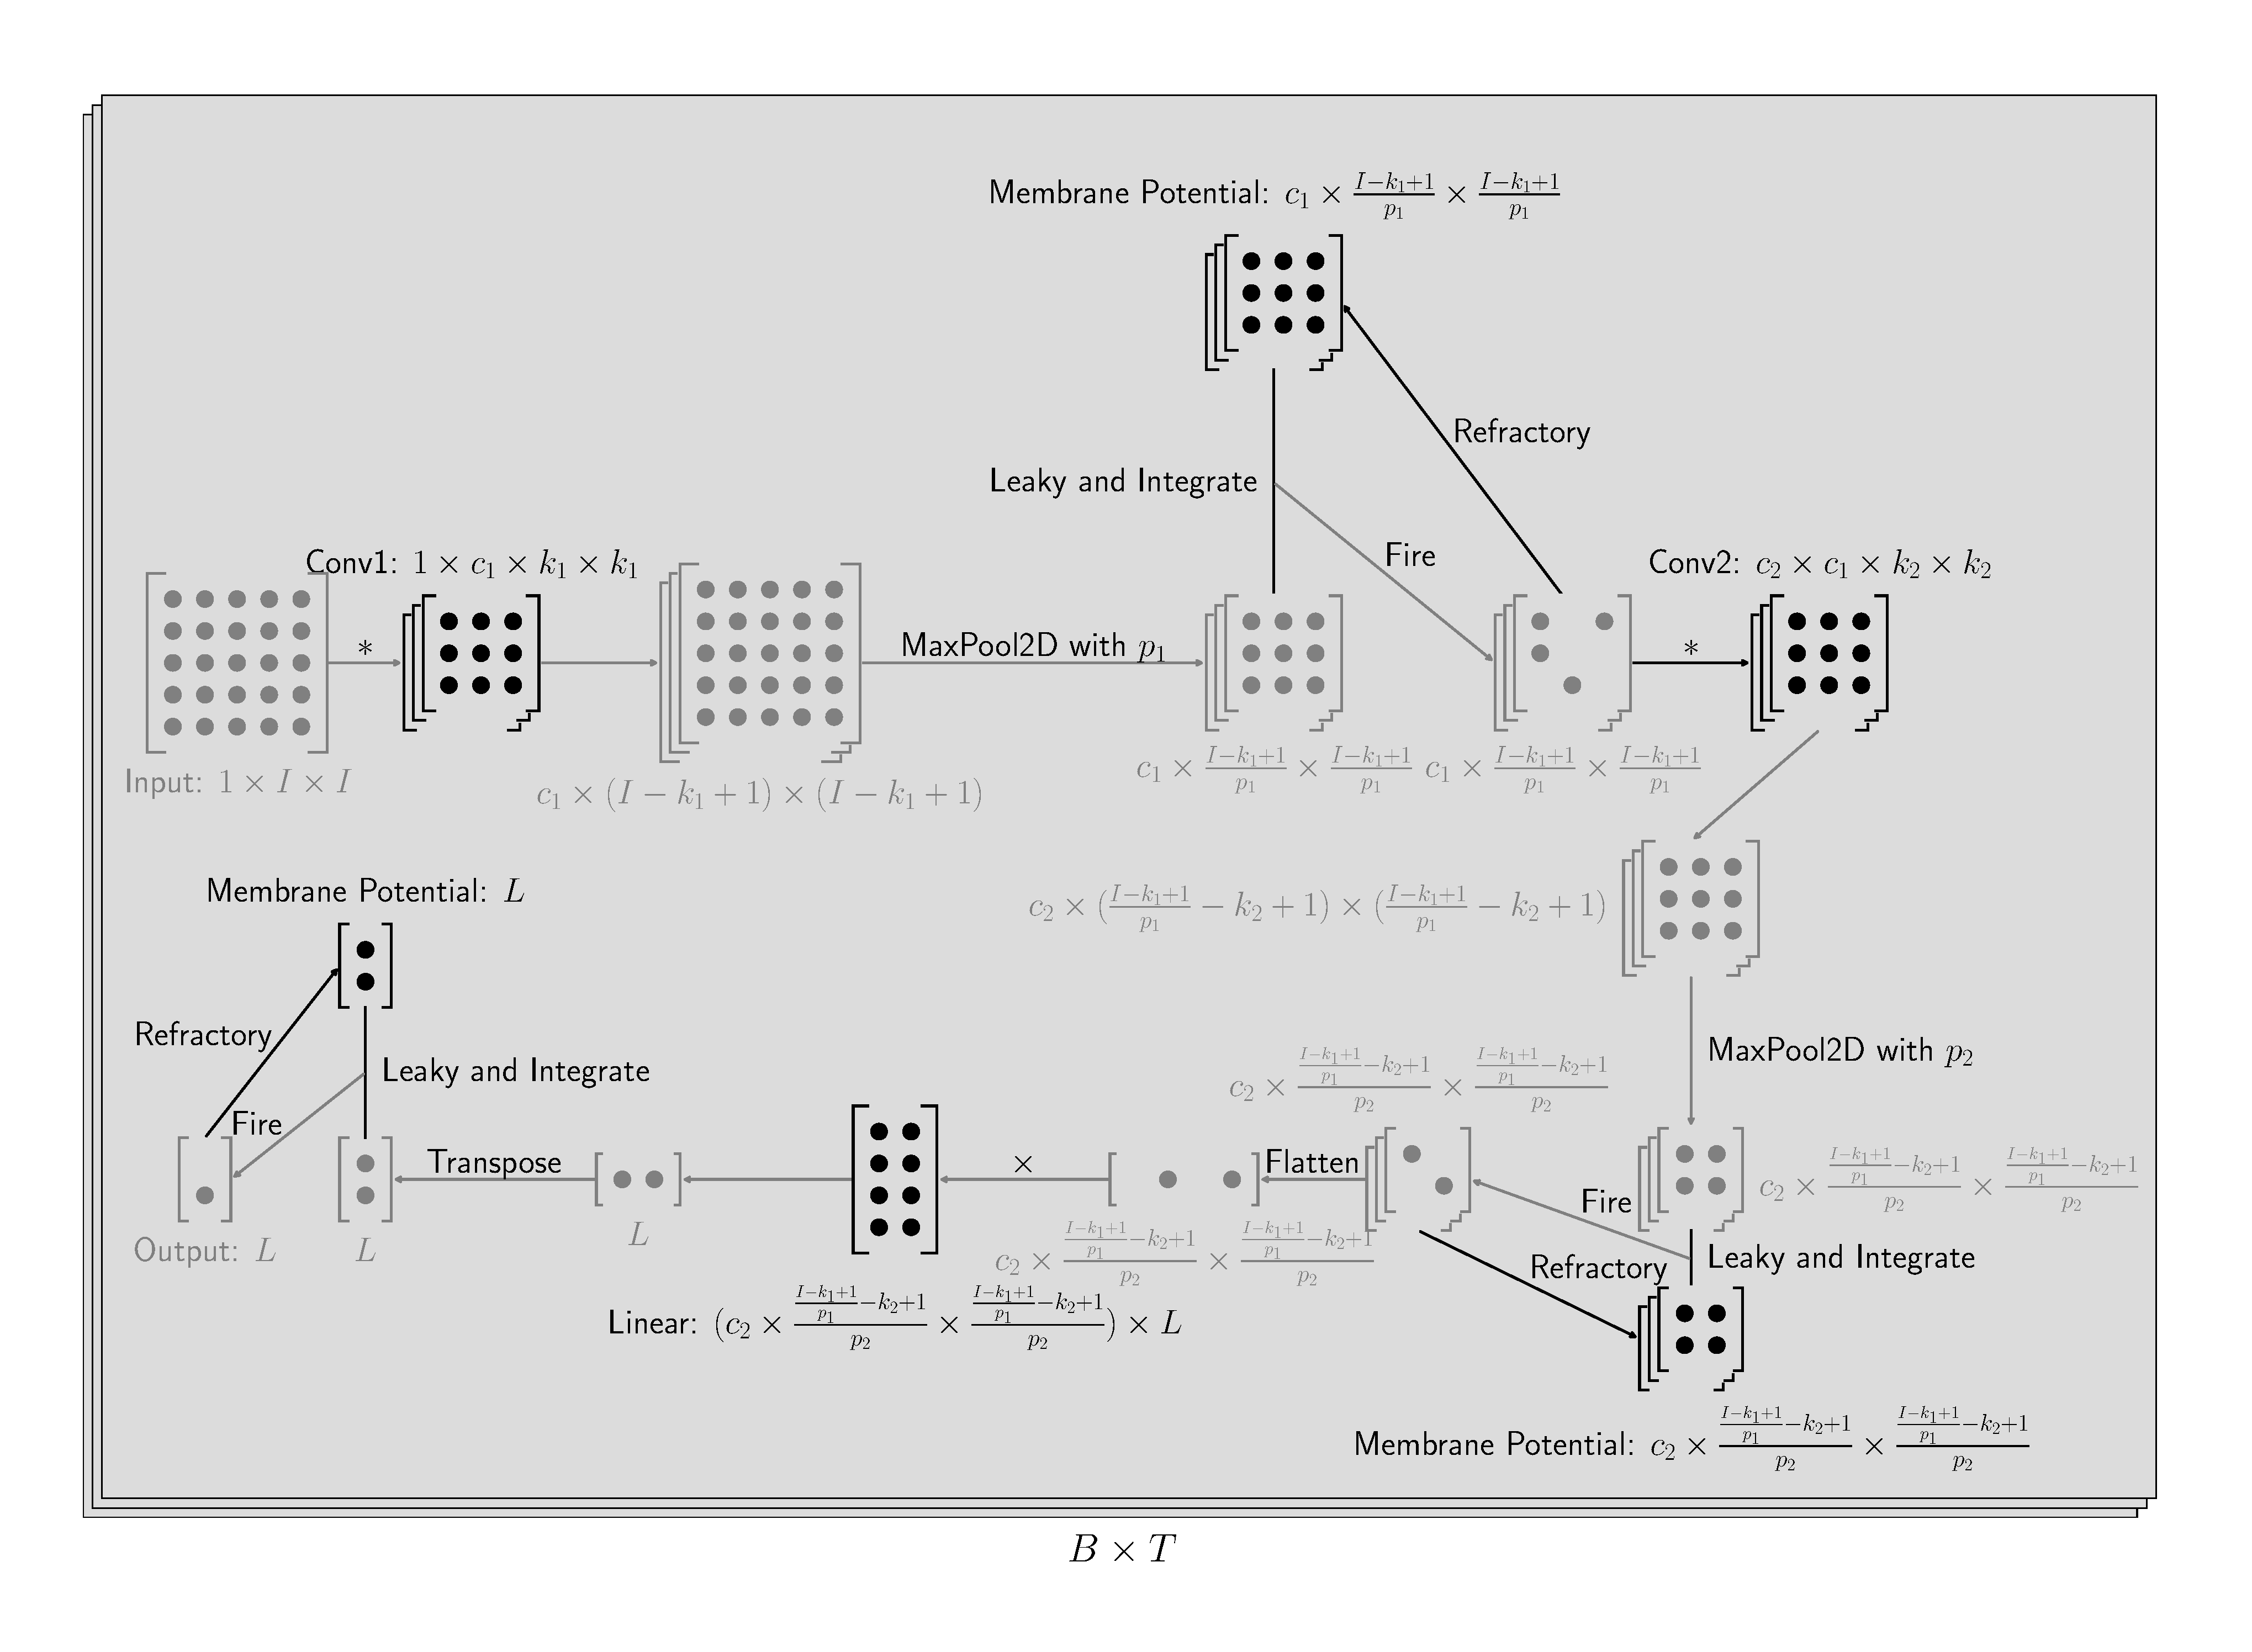
\includegraphics[width=\textwidth]{assets/standard/FashionMNIST/snn2.pdf}
        \caption{The CNN structure used in the experiments with Fashion MNIST dataset}
        \label{fig:scnn_structure}
    \end{figure}

\section{Convergence \& Accuracy}
\label{sec:convergence_accuracy}
    The first noticeable difference between the multi-bit spike train model and the 1-bit spike train model is the convergence speed (see Figure \ref{fig:convergence_speed}). Even just by increasing the bit width of the spike train from 1 to 2, the convergence speed of the network is significantly improved. 
    \begin{figure}[!htpb]
        \centering
        \begin{subfigure}[H]{\textwidth}
            \centering
            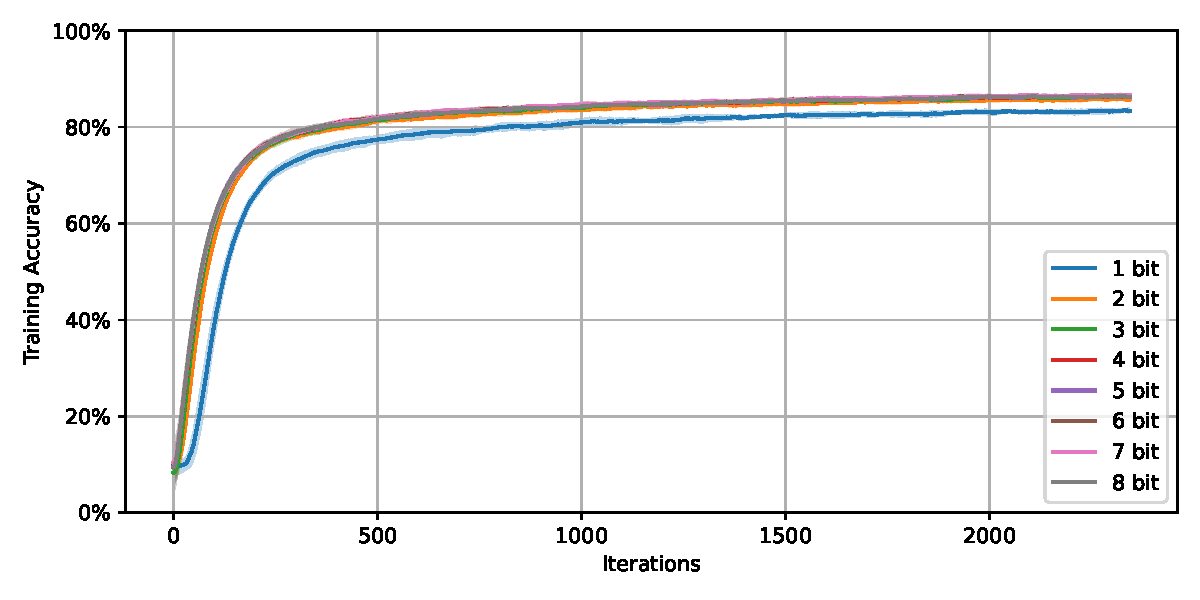
\includegraphics[width=\textwidth]{../standard/FashionMNIST/plots/fashionmnist_train_acc.pdf}
            \caption{Training Accuracy (smoothed with a window size of 100)}
        \end{subfigure}
        \hfill
        \begin{subfigure}[H]{\textwidth}
            \centering
            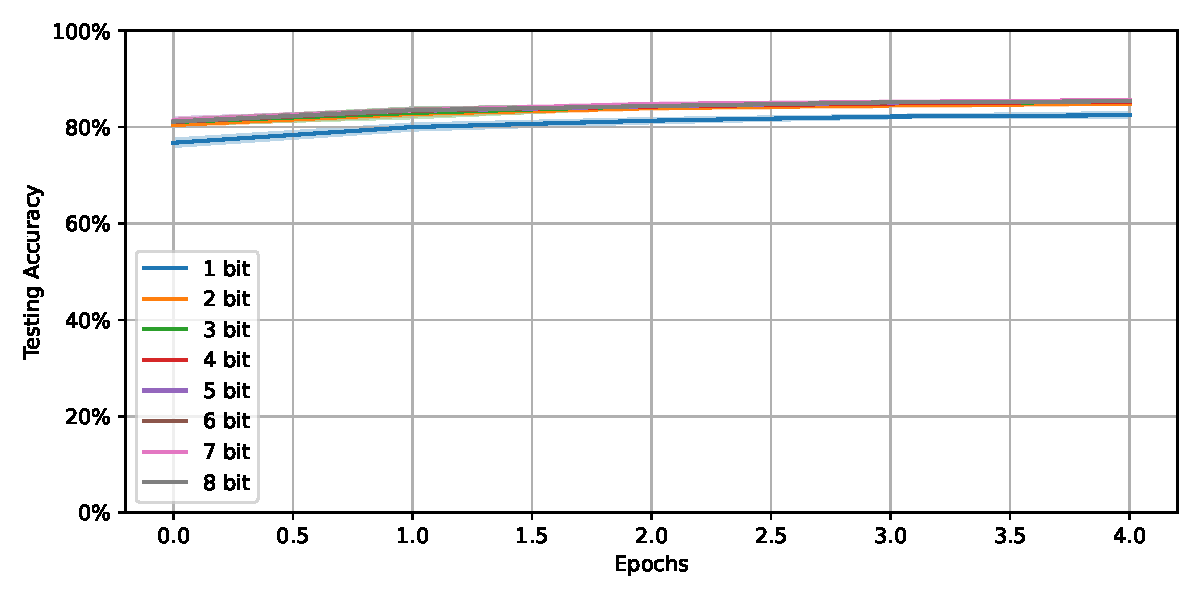
\includegraphics[width=\textwidth]{../standard/FashionMNIST/plots/fashionmnist_test_acc.pdf}
            \caption{Test Accuracy}
        \end{subfigure}
        \caption{Comparison of the Convergence Speed of 1-bit to 8-bit Spike Train Model, repetition of the experiment 10 times}
        \label{fig:convergence_speed}
    \end{figure}

    The improvement in convergence speed can lead to a significant reduction in training time when considering a fixed target accuracy. This is especially noteworthy when considering diminishing returns of accuracy in regards to training time. 

    Here we set the target accuracy to be 80\%. The training time of the multi-bit spike train model is reduced by around 50\%, shown in Figure \ref{fig:iterations_fixed_accuracy}. 
    \begin{figure}[!htpb]
        \centering
        \begin{subfigure}[H]{0.45\textwidth}
            \centering
            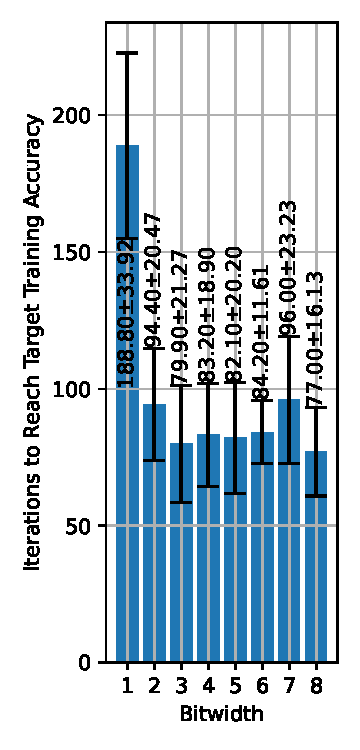
\includegraphics[width=\textwidth]{../standard/FashionMNIST/plots/fashionmnist_train_iters.pdf}
            \caption{Iterations to reach 80\% training accuracy}
        \end{subfigure}
        \hfill
        \begin{subfigure}[H]{0.45\textwidth}
            \centering
            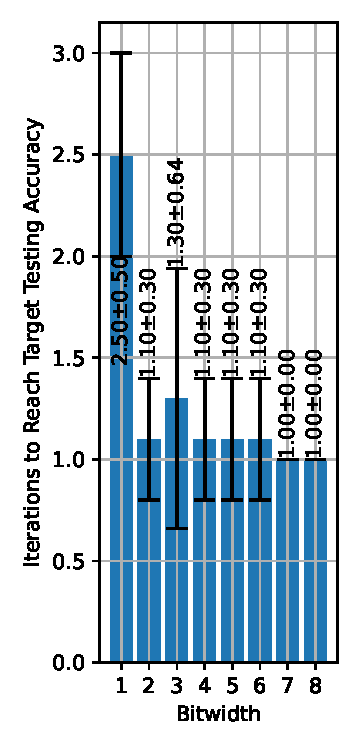
\includegraphics[width=\textwidth]{../standard/FashionMNIST/plots/fashionmnist_test_iters.pdf}
            \caption{Epochs to reach 80\% testing accuracy}
        \end{subfigure}
        \caption{Comparison of the Training Time of 1-bit to 8-bit Spike Train Model, repetition of the experiment 10 times}
        \label{fig:iterations_fixed_accuracy}
    \end{figure}

    This improvement however also comes at certain cost:
    \begin{itemize}
        \item The improvement in convergence speed diminishes as the bit width of the spike train increases. The improvement from 2-bit to 3-bit ($\sim 15.4\%$) or even higher bit width (at most $\sim 59.2\%$ reduction in iterations compared to the 1-bit baseline) is not as significant as the improvement from 1-bit to 2-bit ($\sim 50\%$ reduction in iterations).
        \item The more complicated the model is, the harder is it to train the multi-bit spike train model. One can easily run into the problem of overfitting, for example in the case of DVS gesture recognition task \ref{appendix:accuracy_curves_dvs_gesture}.
    \end{itemize}

    Due to the faster convergence speed, the multi-bit spike train model can achieve better accuracy than the 1-bit spike train model given a fixed number of iterations or epochs for the most cases (see Figure \ref{fig:final_accuracy}).
    \begin{figure}[!htpb]
        \centering
        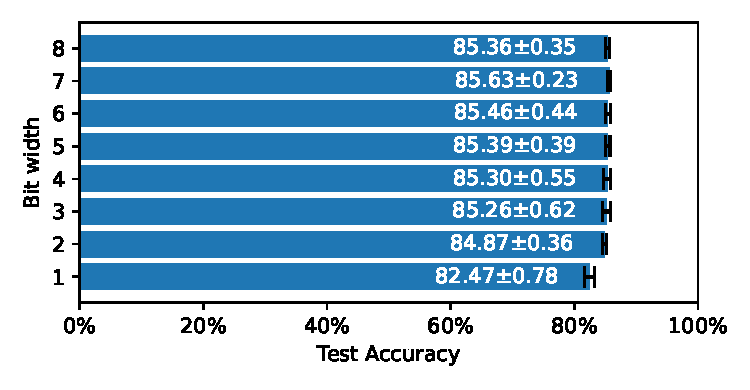
\includegraphics[width=0.8\textwidth]{../standard/FashionMNIST/plots/fashionmnist_final_acc_horizontal.pdf}
        \caption{Comparison of the Final Accuracy of 1-bit to 8-bit Spike Train Model after 5 epochs, repetition of the experiment 10 times}
        \label{fig:final_accuracy}
    \end{figure}

    In general, such behaviors can be shown on MNIST \cite{deng2012mnist}, NMNIST \cite{10.3389/fnins.2015.00437}, Fashion MNIST, DVS gesture recognition \cite{8100264}, and CIFAR-10 datasets (see Appendix \ref{appendix:accuracy}).

\section{Firing Rate}
\label{sec:firing-rate}
    SNNs are known for their sparsity in the firing rate of the neurons. Here we notice that the multi-bit spike train model has a higher firing rate than the 1-bit spike train model (see Figure \ref{fig:firing_rate}), as tradeoff for the improvement in convergence speed. 
    \begin{figure}[!htpb]
        \centering
        \begin{subfigure}[H]{0.9\textwidth}
            \centering
            \includegraphics[width=\textwidth]{../standard/FashionMNIST/plots/fashionmnist_train_firerate.pdf}
            \caption{Training Firing Rate}
        \end{subfigure}
    \end{figure}
    \begin{figure}[!htpb]
        \ContinuedFloat
        \begin{subfigure}[H]{0.9\textwidth}
            \centering
            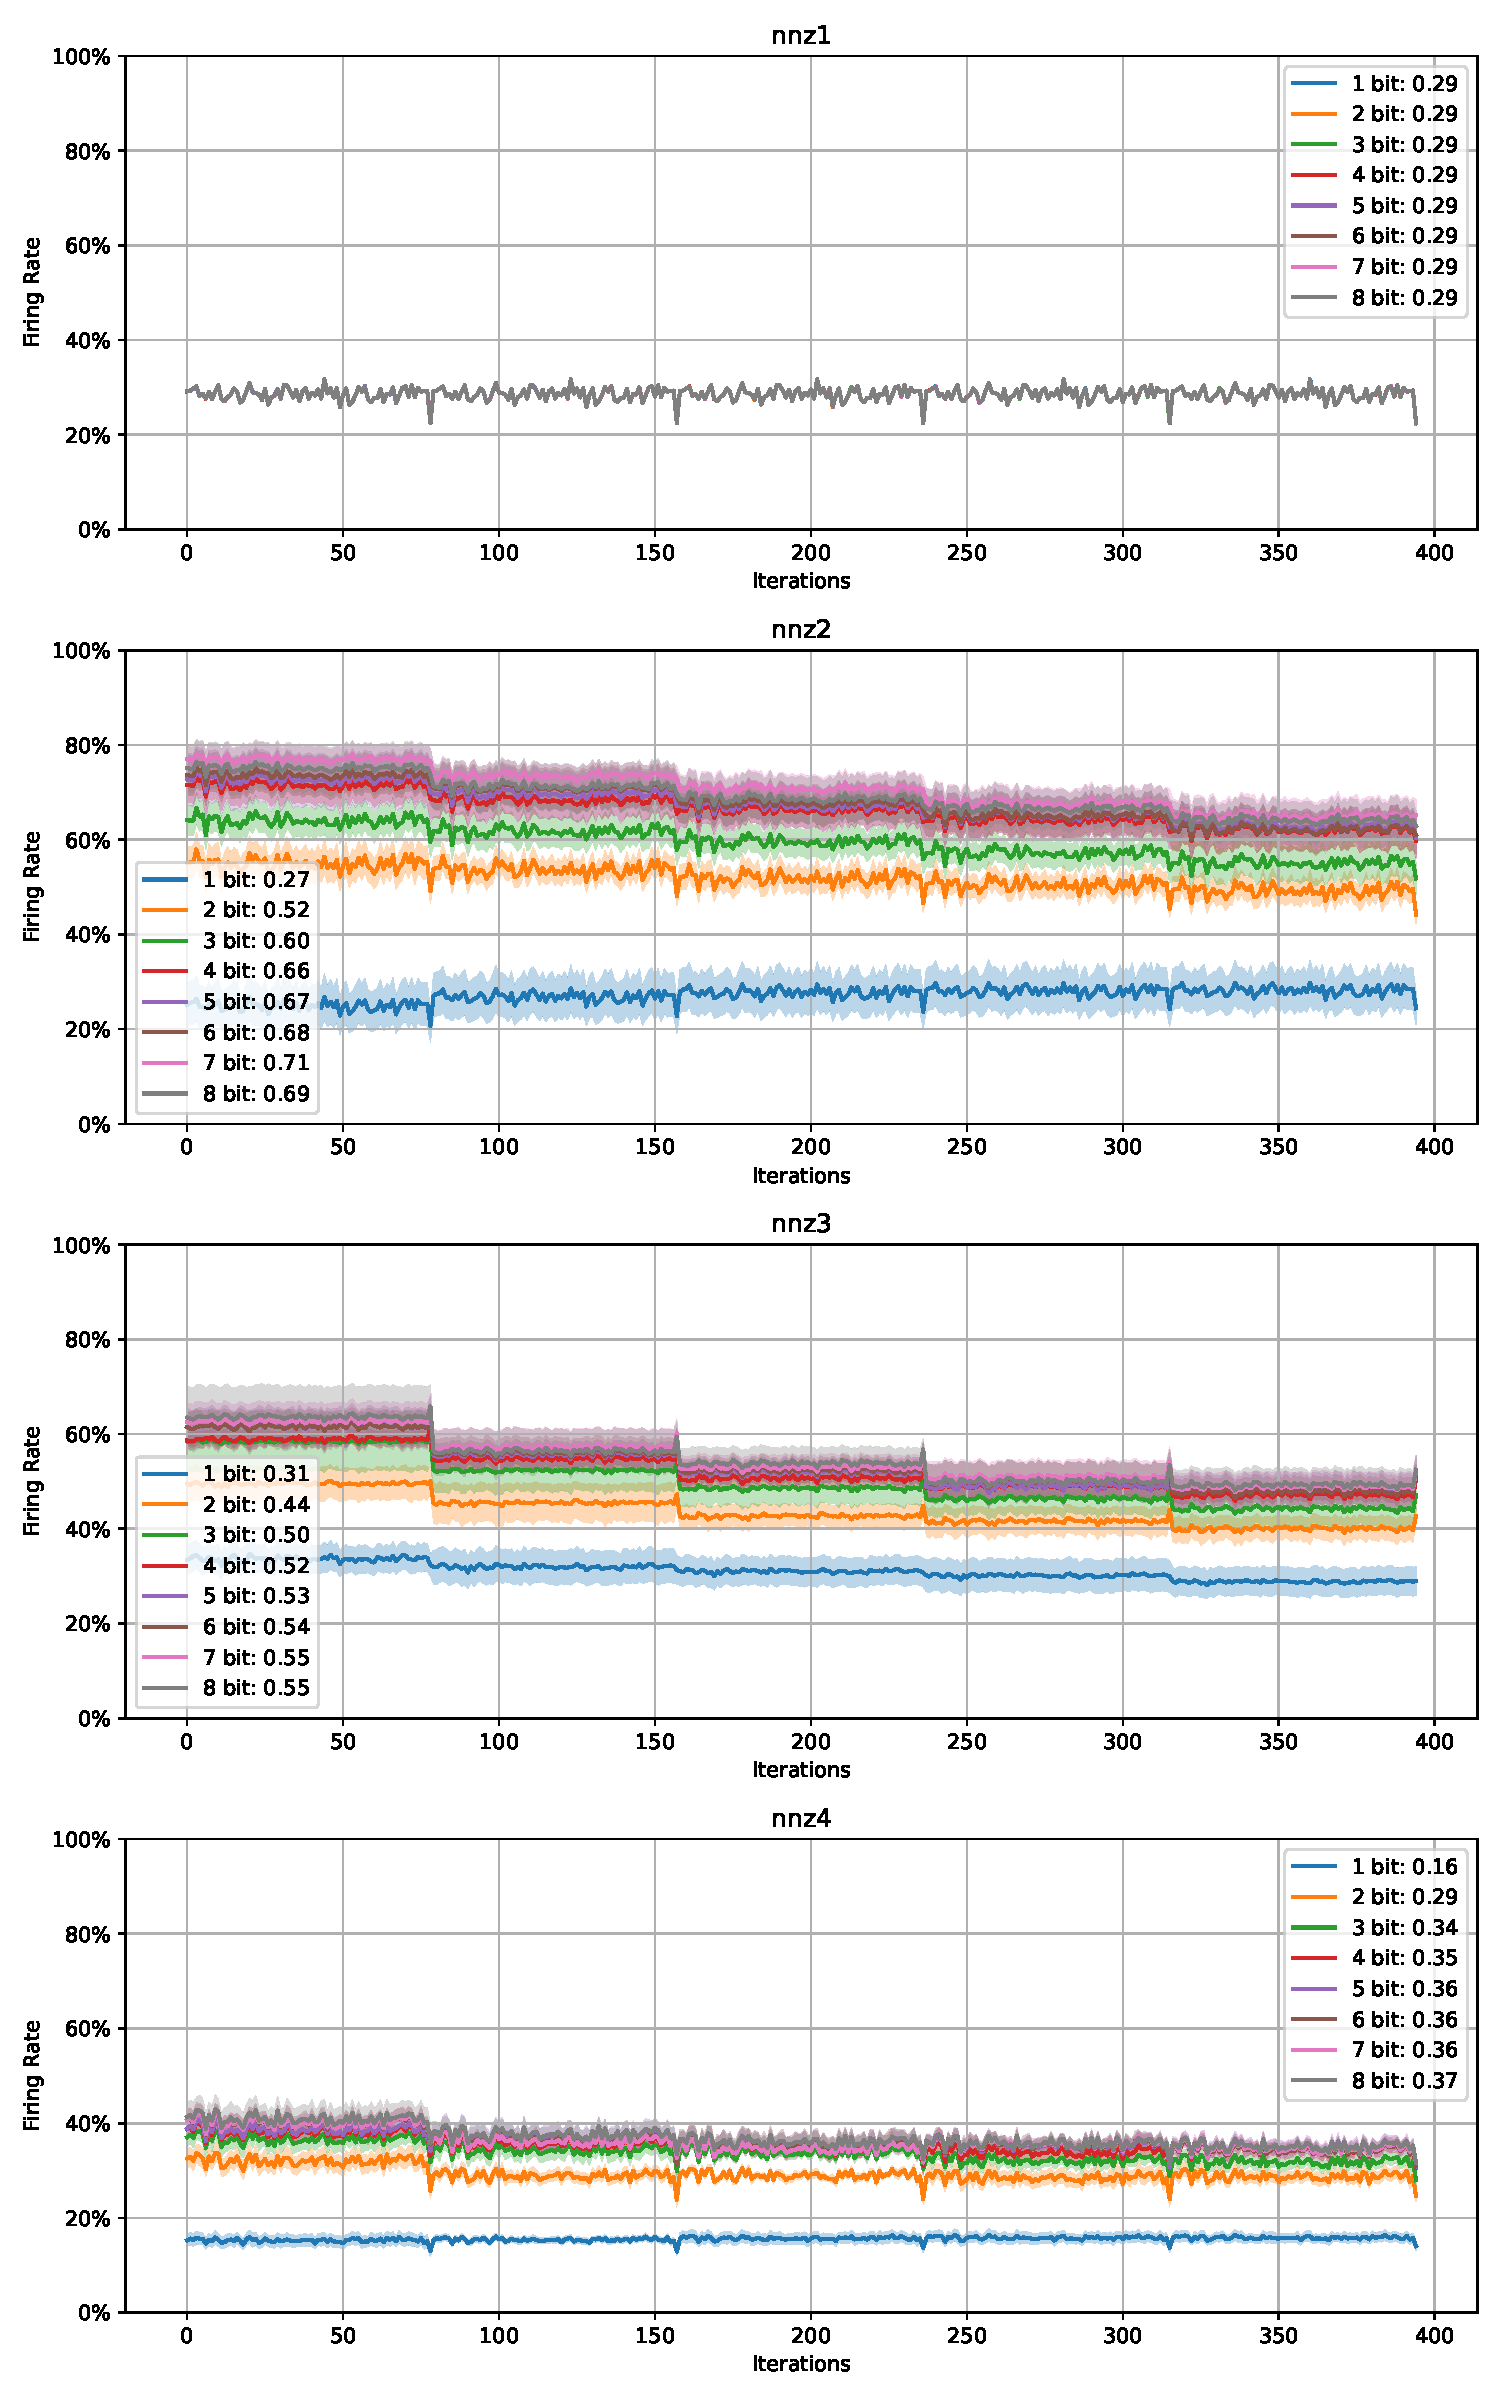
\includegraphics[width=\textwidth]{../standard/FashionMNIST/plots/fashionmnist_test_firerate.pdf}
            \caption{Test Firing Rate}
        \end{subfigure}
        \caption{Comparison of the Firing Rate of 1-bit to 8-bit Spike Train Model: repetition of the experiment 10 times, "nnz[i]" means the number of non-zero elements in the $i$-th measuring point, corresponding to the position from the inputs to the output layer, "nnz1" is the input data}
        \label{fig:firing_rate}
    \end{figure}

    One can notice that the firing rate of the multi-bit spike train model peaks at the very beginning of the training session, when the model converges rapidly. The firing rate then decreases as the training progresses. If we extend the training session, the firing rate of the multi-bit spike train model tends to converge to the firing rate of the 1-bit spike train model. However, such process takes however a long time (see Figure \ref{fig:long_firing_rate}). 
    \begin{figure}[!htpb]
        \centering
        \begin{subfigure}[H]{0.9\textwidth}
            \centering
            \includegraphics[width=\textwidth]{../firerate/FashionMNIST/plots/fashionmnist_train_firerate.pdf}
            \caption{Training Firing Rate}
        \end{subfigure}
    \end{figure}
    \begin{figure}[!htpb]
        \ContinuedFloat
        \begin{subfigure}[H]{0.9\textwidth}
            \centering
            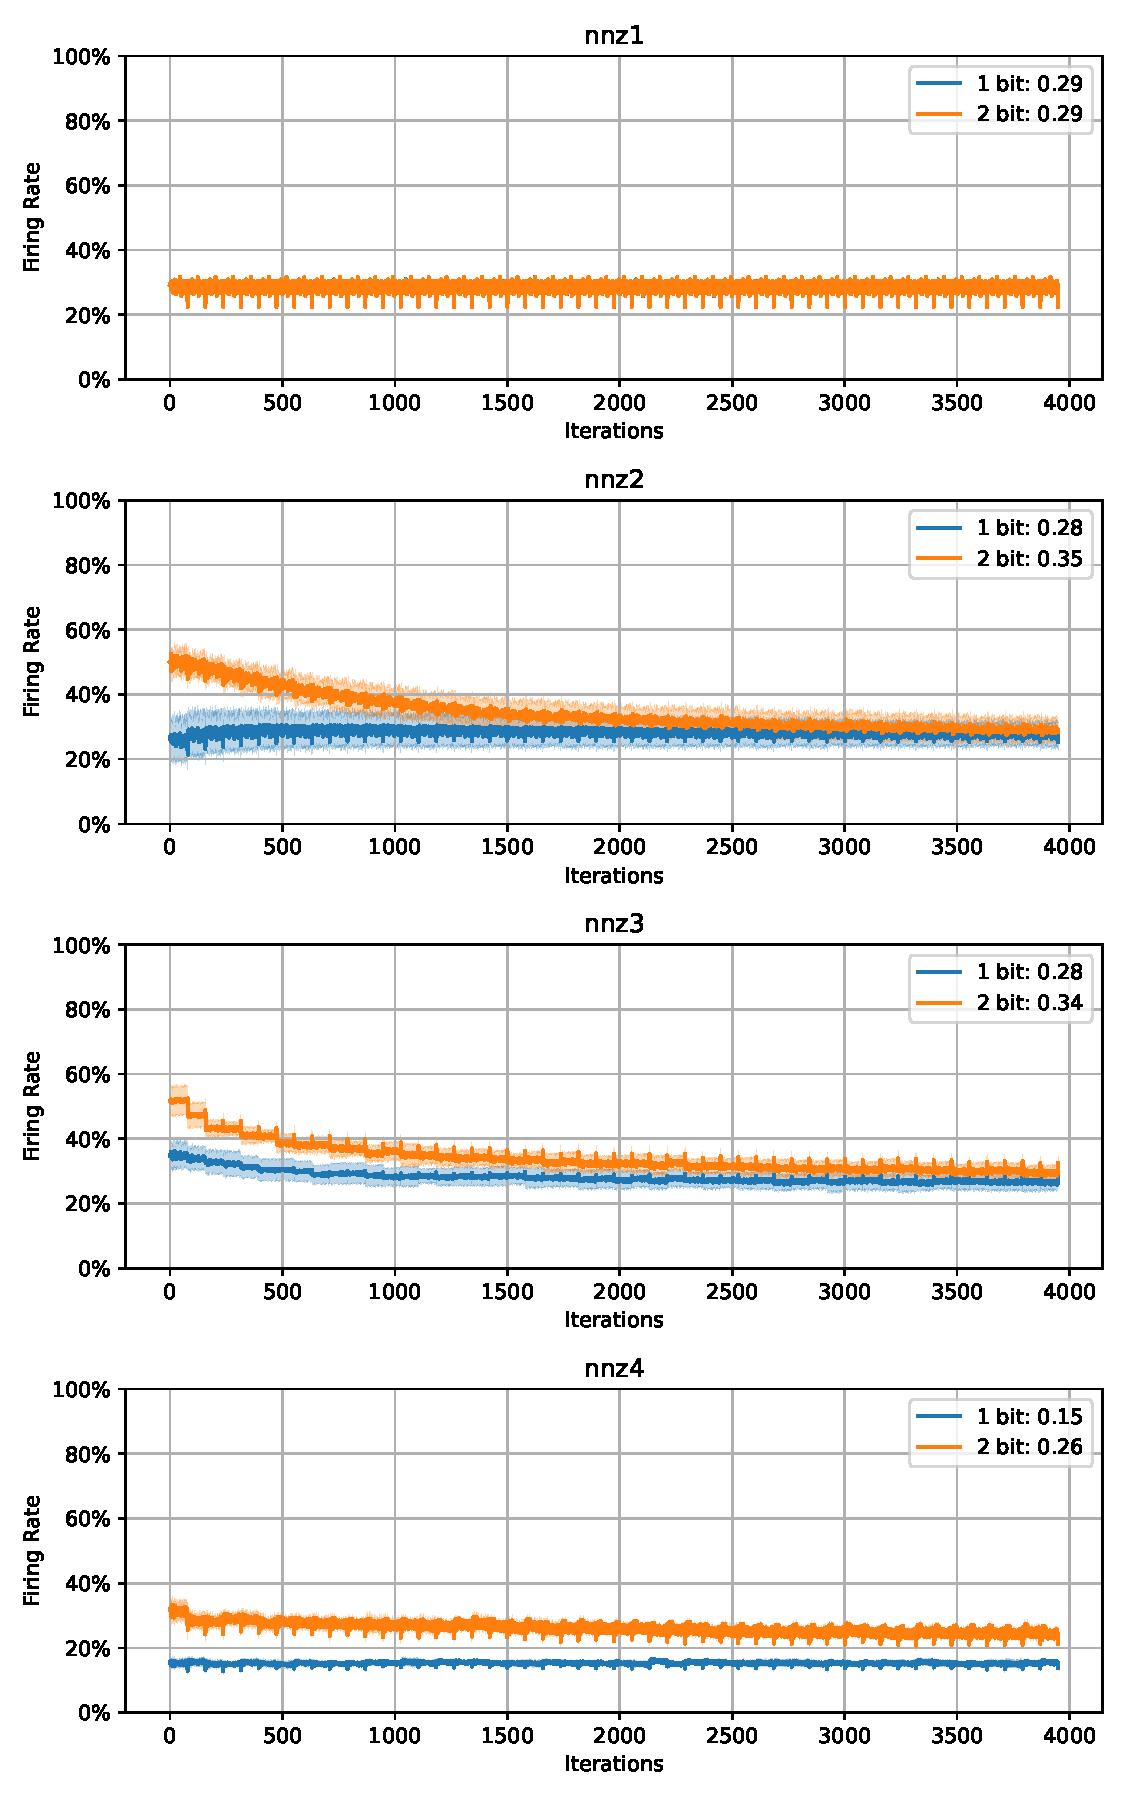
\includegraphics[width=\textwidth]{../firerate/FashionMNIST/plots/fashionmnist_test_firerate.pdf}
            \caption{Test Firing Rate}
        \end{subfigure}
        \caption{Analog to figure \ref{fig:firing_rate}, but with a training session of 50 epochs instead of 5 epochs, only the 1-bit and 2-bit spike train models}
        \label{fig:long_firing_rate}
    \end{figure}

    Towards the end of the training time, the firing rate of the multi-bit spike train model is comparable to the 1-bit spike train model (see Figure \ref{fig:final_firing_rate}).
    \begin{figure}[!htpb]
        \centering
        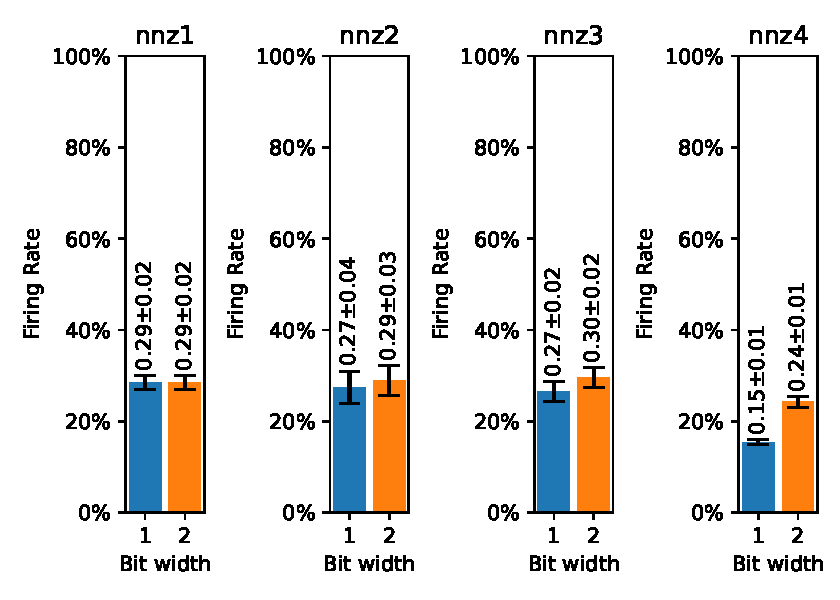
\includegraphics[width=\textwidth]{../firerate/FashionMNIST/plots/fashionmnist_final_firerate.pdf}
        \caption{Comparison of the Final Firing Rate of 1-bit to 8-bit Spike Train Model after 50 epochs, only the 1-bit and 2-bit spike train models}
        \label{fig:final_firing_rate}
    \end{figure}

    Such behavior is more visible on simpler datasets like MNIST. For now, we do not have any explanation for this phenomenon (see Appendix \ref{appendix:firerate}).

\section{Quantizability}
\label{sec:quantizability}
    A common technique to reduce the memory footprint of SNNs without having significant impact on accuracy is quantization \cite{9534087}. There are studies showing that the weights and activations of SNNs can be quantized to 1-bit or 2-bit without significant loss in accuracy \cite{10.1145/3664647.3681186}. Here we show that both the multi-bit spike train model and the 1-bit spike train model can be trained with \verb|bf16| and quantized to \verb|int8| without significant loss in accuracy.
    % TODO: Add references to the studies showing the quantizability of SNNs
    \begin{figure}[!htpb]
        \centering
        \begin{subfigure}[H]{0.89\textwidth}
            \centering
            \begin{subfigure}[H]{\textwidth}
                \centering
                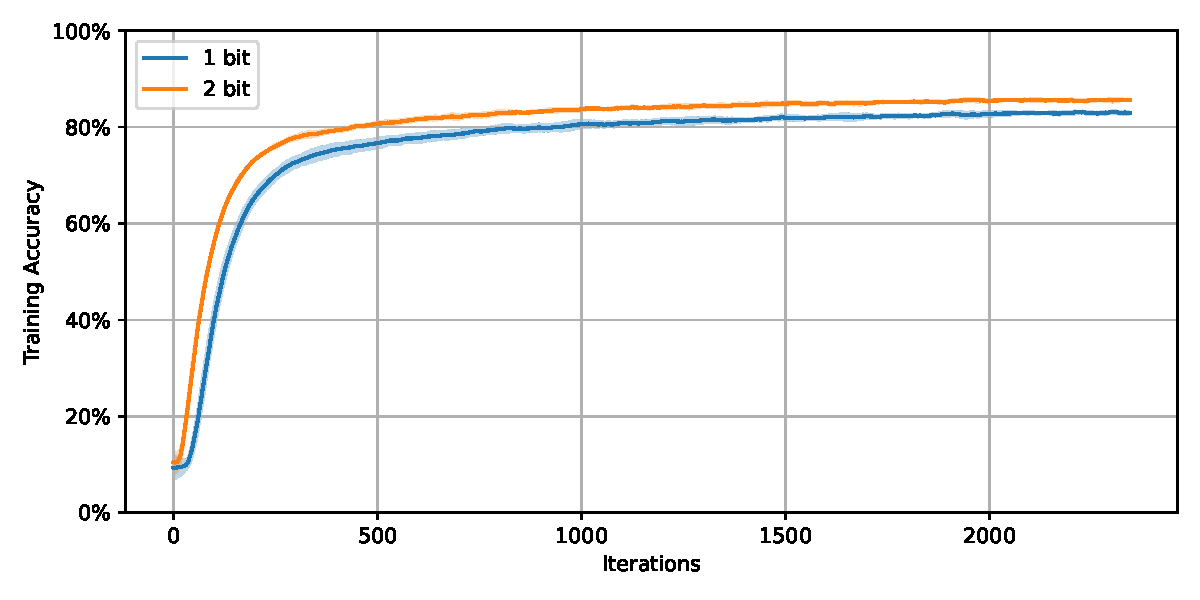
\includegraphics[width=\textwidth]{../quantized/FashionMNIST/plots/fashionmnist_train_acc.pdf}
                \caption{Training Accuracy with half precision (smoothed with a window size of 100)}
            \end{subfigure}
            \hfill
            \begin{subfigure}[H]{\textwidth}
                \centering
                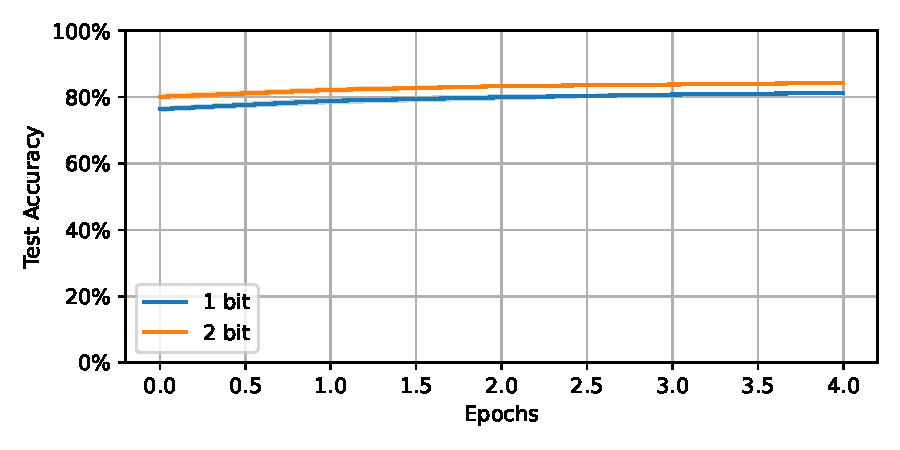
\includegraphics[width=\textwidth]{../bf16/FashionMNIST/plots/fashionmnist_test_acc.pdf}
                \caption{Test Accuracy with half precision}
            \end{subfigure}
        \end{subfigure}
        \hfill
        \begin{subfigure}[H]{0.1\textwidth}
            \centering
            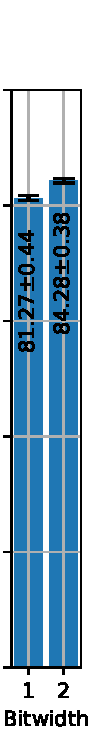
\includegraphics[width=\textwidth]{../bf16/FashionMNIST/plots/fashionmnist_final_acc.pdf}
            \caption{Final Accuracy with half precision after 5 epochs}
        \end{subfigure}
        \caption{Comparison of the Convergence Speed of 1-bit to 8-bit Spike Train Model with half precision, repetition of the experiment 10 times}
        \label{fig:half_precision}
    \end{figure}

    As shown in Figure \ref{fig:half_precision}, both SNN models converge well as if they were trained with \verb|float32|. Meanwhile the multi-bit spike train model has its advantage in the convergence speed and accuracy preserved. 
    
    Before quantizing the models to \verb|int8|, we first apply quantization-aware training to both SNN models. While regular ANNs may encounter various problems due to the high sensitivity in inputs and parameters, both SNN models here converge well. We also see that the multi-bit spike train model has a faster convergence speed and better accuracy than the 1-bit spike train model (Figure \ref{fig:quantization_aware}). 
    \begin{figure}[!htpb]
        \centering
        \begin{subfigure}[H]{0.89\textwidth}
            \centering
            \begin{subfigure}[H]{\textwidth}
                \centering
                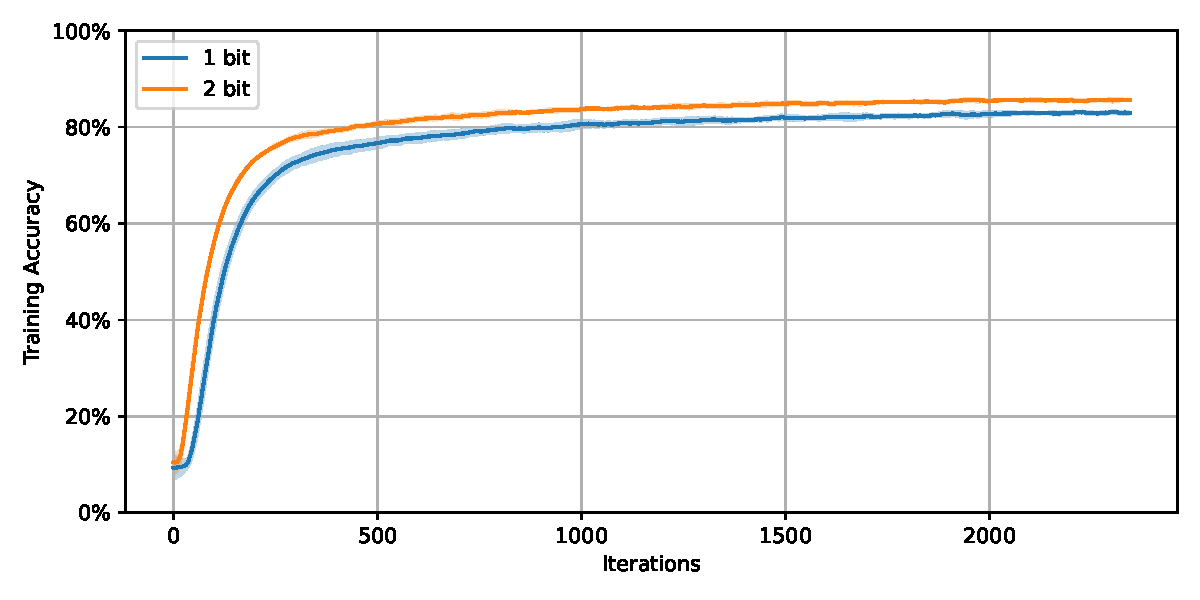
\includegraphics[width=\textwidth]{../quantized/FashionMNIST/plots/fashionmnist_train_acc.pdf}
                \caption{Training Accuracy with quantization-aware training (smoothed with a window size of 100)}
            \end{subfigure}
            \hfill
            \begin{subfigure}[H]{\textwidth}
                \centering
                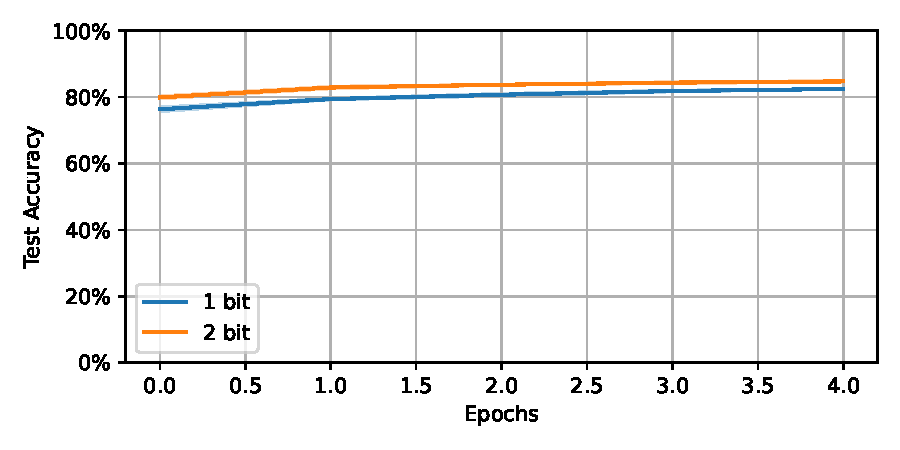
\includegraphics[width=\textwidth]{../quantized/FashionMNIST/plots/fashionmnist_test_acc.pdf}
                \caption{Test Accuracy with quantization-aware training}
            \end{subfigure}
        \end{subfigure}
        \hfill
        \begin{subfigure}[H]{0.1\textwidth}
            \centering
            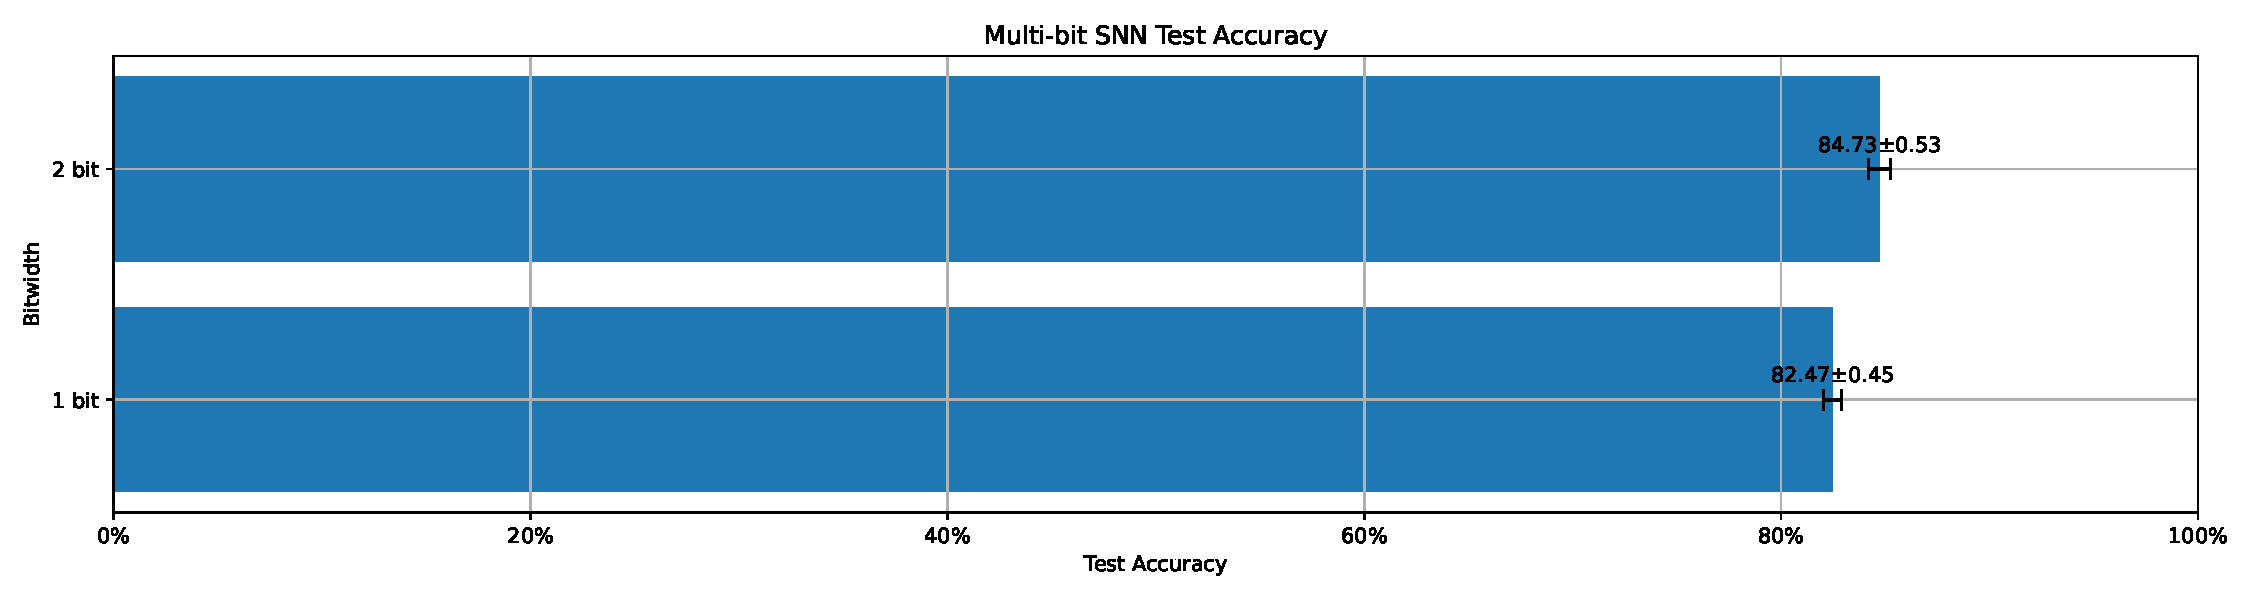
\includegraphics[width=\textwidth]{../quantized/FashionMNIST/plots/fashionmnist_final_acc.pdf}
            \caption{Final Accuracy with quantization-aware training after 5 epochs}
            \label{fig:quantization_aware_final_acc}
        \end{subfigure}
        \caption{Comparison of the Convergence Speed of 1-bit to 8-bit Spike Train Model with quantization-aware training, repetition of the experiment 10 times}
        \label{fig:quantization_aware}
    \end{figure}

    We then quantize the weights and biases to \verb|int8| using the PyTorch quantization API. The quantization of the LIF layer is not supported at the moment. We evaluate the quantized models on the test set. The final accuracy is barely affected by the quantization (see Figure \ref{fig:quantization_aware_final_acc}). 

\section{Energy Consumption}
\label{sec:energy-consumption}
    One of the main motivations for SNNs is their energy efficiency compared to ANNs on specialized hardware like neuromorphic chips. Products like Loihi from Intel \cite{8259423} and TrueNorth from IBM \cite{7229264} have proved the potential of SNNs by utilizing the asynchronous communication via spikes. In the real-world scenario, one often uses accelerators like GPUs to train SNNs and deploy them on specialized hardware to achieve fast training and energy efficent inference. 

    Here we present an energy consumption model for the multi-bit spike train model and compare it with the 1-bit spike train model. We consider the unique properties of various hardware implementations and give the energy consumption of the multi-bit spike train model relative to the 1-bit spike train model. 

    \subsection{Training Energy Consumption on GPUs}
    \label{subsec:training_energy}
        On GPUs, low precision spikes are generally not very meaningful, as the hardware is not designed for such level mixed precision operations. Often the spikes are represented as 32-bit floating point numbers, which can be computed with the weights with the same precision. Popular SNN frameworks like snnTorch and SpikingJelly do not utilize the sparsity of spike trains. So in this case, the firing rate and the bit width of the spike train do not affect the energy consumption of the training phase. 
    
        The only factors that matter are the number of iterations required to reach a certain accuracy and the number of time steps that the network is simulated, assuming fixed network topology and batch size. 
    
        This allows us to create a simple, yet effective energy consumption model for the training phase on the GPUs. Let $T_i$ denote the number of time steps, $S_i$ denote the number of iterations required to reach a certain accuracy, and $E_{\text{train}-i}$ denote the energy consumption. Then we have:
        \begin{equation}
            E_{\text{train}-i} = T_i \cdot S_i \cdot c
        \end{equation}
        where $c$ is a constant factor that depends on the hardware and the software used, yet remains the same across different bit widths of the spike train. 
    
        As noticed in Section \ref{sec:convergence_accuracy}, one requires fewer iterations to reach a certain accuracy with the multi-bit spike train model. Here we focus on the energy consumption of the 2-bit spike train model, as it does not increase the firing rate as much as the other higher bit width models while still providing a significant improvement in convergence speed and accuracy. 

        Based on the results in Section \ref{fig:iterations_fixed_accuracy}, we can estimate the energy consumption of the 2-bit spike train model relative to the 1-bit spike train model directly by comparing the number of iterations required to reach a certain accuracy which is around $50.00\pm10.84\%$ in this case (see Figure \ref{fig:training_energy_gpu}). 
        \begin{figure}[!htpb]
            \centering
            \begin{subfigure}[H]{0.45\textwidth}
                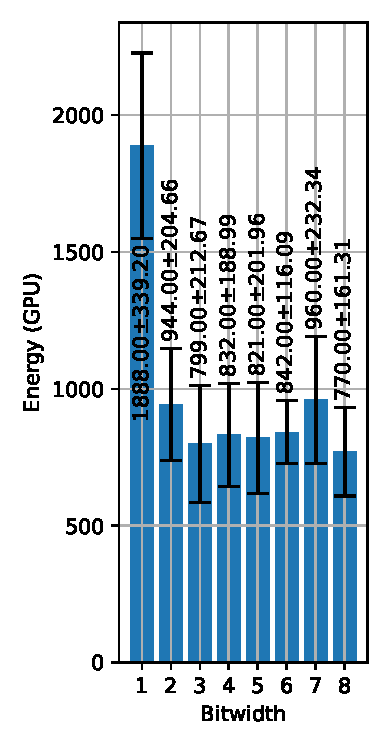
\includegraphics[width=\textwidth]{../standard/FashionMNIST/plots/fashionmnist_train_energy_gpu.pdf}
                \caption{Energy Consumption Estimation, Unit in Constant $c$}
            \end{subfigure}
            \hfill
            \begin{subfigure}[H]{0.45\textwidth}
                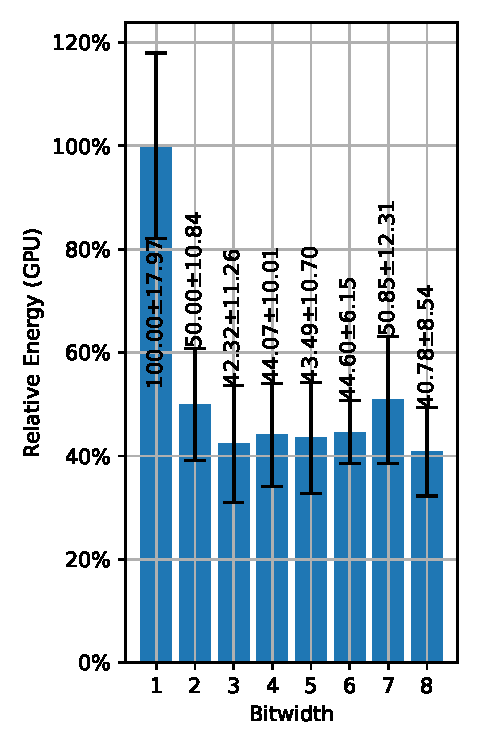
\includegraphics[width=\textwidth]{../standard/FashionMNIST/plots/fashionmnist_train_relative_energy_gpu.pdf}
                \caption{Normalized Energy Consumption Estimation Relative to 1-bit Spike Train Model}
            \end{subfigure}
            \caption{Training Energy Consumption Estimation on GPUs for Fashion MNIST Dataset}
            \label{fig:training_energy_gpu}
        \end{figure}

        More details with other datasets (MNIST, NMNIST, DVS Gesture and CIFAR10) can be found in Appendix \ref{appendix:energy_gpu}.

    \subsection{Inference Energy Consumption on Neuromorphic Chips}
    \label{subsec:inference_energy}
        A widely adopted (e.g. in \cite{zhu2024spikegptgenerativepretrainedlanguage} and \cite{chen2024deepreinforcementlearningspiking}) energy estimation model for neuromorphic chips is the following:
        \begin{equation}
            \label{eq:inference_energy_popular}
            E_{\text{inference}} \approx F \cdot fr \cdot E_{\text{AC}} \cdot T
        \end{equation}
        where $F$ is the number of floating point operations required to simulate the network, $fr$ is the firing rate of the input neurons, $E_{\text{AC}}$ is the energy consumption of accumulation, and $T$ is the number of time steps. 
    
        Despite this, it is difficult to evaluate the energy consumption of the multi-bit spike train model on neuromorphic chips like Loihi and TrueNorth, as they do not support multi-bit spikes natively. Although it may be possible to encode the multi-bit spikes into multiple spikes with different intensities, the energy consumption of such encoding would be very expensive due to the high cost of the synchronization barrier between the time steps. 

        A viable option would be to consider hardware like Intel Loihi 2 which supports graded spikes up to 32-bit precision. We consider the case of Intel Loihi 2 and make the following assumptions: 
        \begin{enumerate}
            \item There is no difference in the energy consumption for the number of bits used to encode the spikes.
            \item The neuromorphic hardware performs add-and-accumulate operations whenever a spike is received. 
        \end{enumerate}
        Since the payload is not variable in this case, the energy consumption of the multi-bit spike train model is directly proportional to the firing rate given a fixed maximum number of floating point operations and time steps. Analogously to the equation \ref{eq:inference_energy_popular}, we have the following estimation for the $i$-bit spike train model:
        \begin{equation}
            E_{\text{inference}-i} \approx F \cdot fr_i \cdot E_{\text{AC}} \cdot T_i
        \end{equation}
        We can estimate the energy consumption of the 2-bit spike train model relative to the 1-bit spike train model by comparing the firing rate of the neurons. As expected, the energy consumption of the multi-bit spike train model is higher than the 1-bit spike train model, as the firing rate of the neurons is higher (see Figure \ref{fig:inference_energy_nh}).
        \begin{figure}[!htpb]
            \centering
            \begin{subfigure}[H]{0.48\textwidth}
                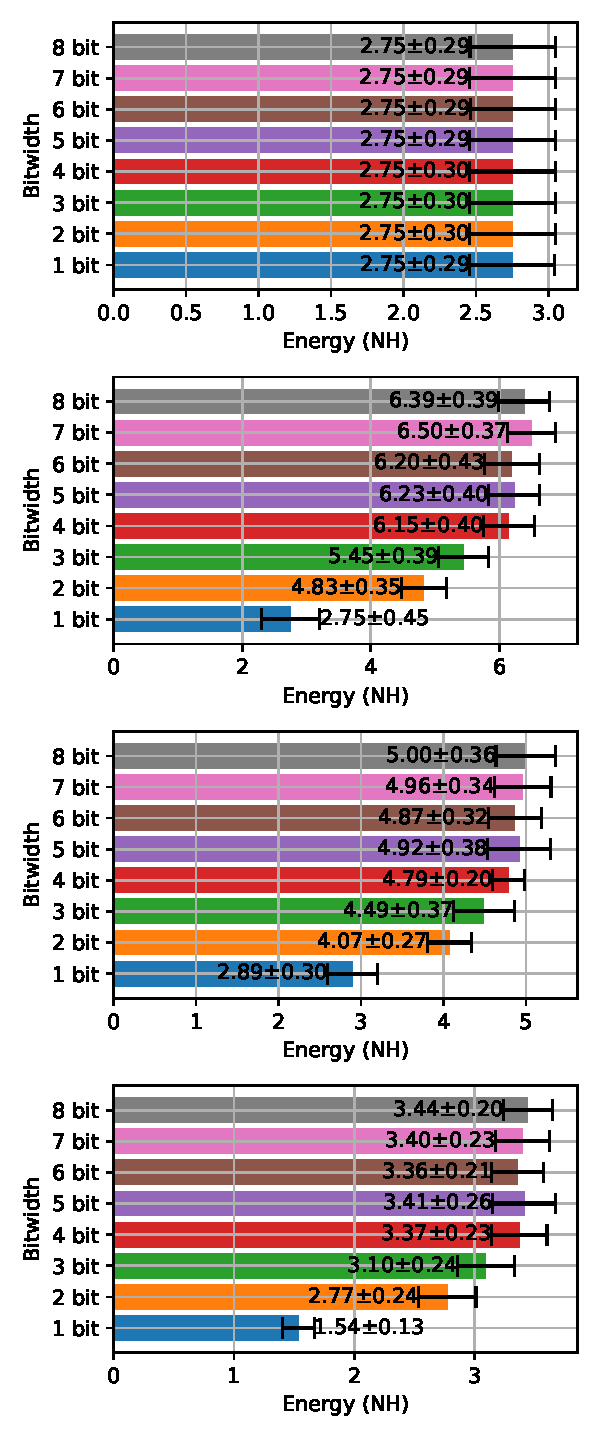
\includegraphics[width=\textwidth]{../standard/FashionMNIST/plots/fashionmnist_test_energy_nh.pdf}
                \caption{Energy Consumption Estimation, Unit in Parameters $F\cdot E_{\text{AC}}$}
            \end{subfigure}
            \hfill
            \begin{subfigure}[H]{0.48\textwidth}
                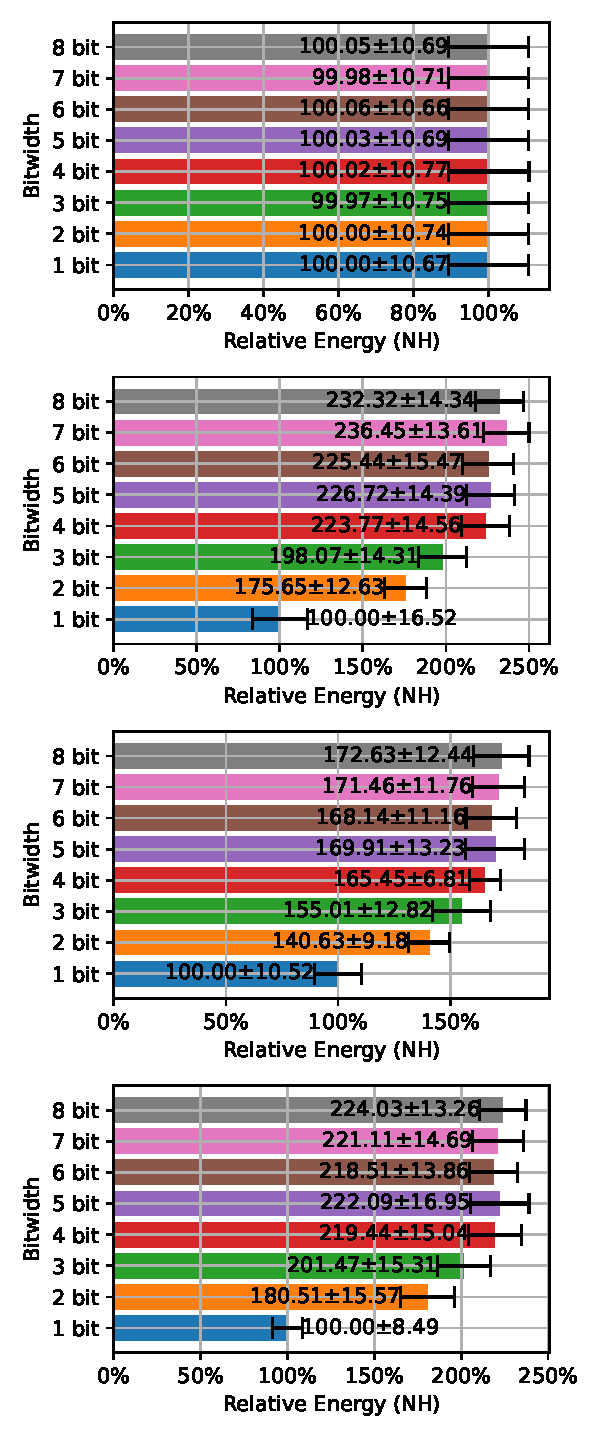
\includegraphics[width=\textwidth]{../standard/FashionMNIST/plots/fashionmnist_test_relative_energy_nh.pdf}
                \caption{Normalized Energy Consumption Estimation Relative to 1-bit Spike Train Model}
            \end{subfigure}
            \caption{Inference Energy Consumption Estimation on Intel Loihi 2 for Fashion MNIST Dataset}
            \label{fig:inference_energy_nh}
        \end{figure}

        More details with other datasets (MNIST, NMNIST, DVS Gesture and CIFAR10) can be found in Appendix \ref{appendix:energy_neuromorphic}.
        %TODO: Add references to the analysis model

        We consider $E_{\text{AC}}=0.9\text{pJ}$, $E_{\text{MAC}}=4.5\text{pJ}$ (energy cost for multiply-and-accumulate operations) \cite{6757323} to estimate the precise energy consumption of the multi-bit spike train model and the ANN for Fashion MNIST dataset (see Figure \ref{fig:energy_ann_vs_snn}). Due to the small network size and the high firing rate, the energy consumption of the multi-bit spike train model is higher than the ANN in some cases.
        \begin{figure}[!htpb]
            \centering
            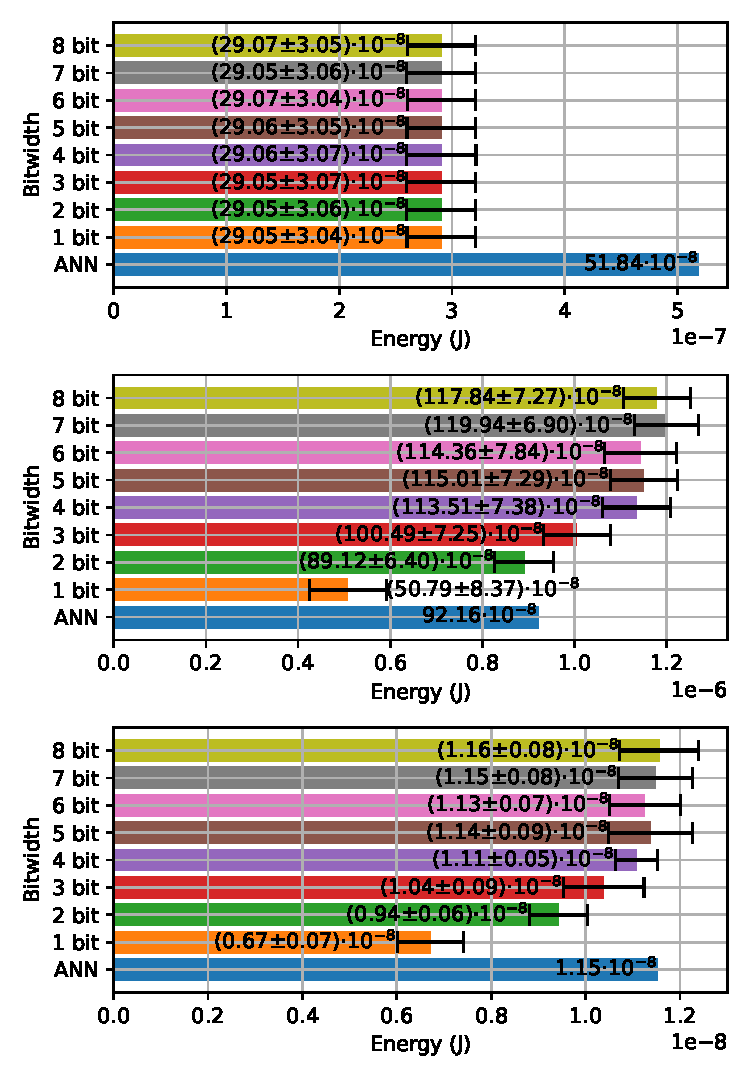
\includegraphics[width=0.6\textwidth]{../standard/FashionMNIST/plots/fashionmnist_energy_ann_vs_snn.pdf}
            \caption{Comparison of the Energy Consumption of ANN and Multi-Bit Spike Train Model on Intel Loihi 2 for Fashion MNIST Dataset, from top to bottom: first convolution block, second convolution block, output layer}
            \label{fig:energy_ann_vs_snn}
        \end{figure}

    \subsection{Tradeoffs}
        One can tell that the energy consumption of the multi-bit spike train model has no direct advantage over the 1-bit spike train model on neuromorphic chips, as the firing rate of the multi-bit spike train model tends to be higher than the 1-bit spike train model. 

        We consider the energy consumption of the multi-bit spike train model in general as an opportunity to enable tradeoffs. If the inference is not the bottleneck of the application, then one can rely on the fast convergence speed of the multi-bit spike train model during training. If the inference is the bottleneck, then one can choose to train the multi-bit spike train model for longer time to achieve a firing rate that is comparable to the 1-bit spike train model (see Figure \ref{fig:inference_energy_nh_firerate}). Such tradeoffs are not possible with the 1-bit spike train model. 
        \begin{figure}[!htpb]
            \centering
            \begin{subfigure}[H]{0.48\textwidth}
                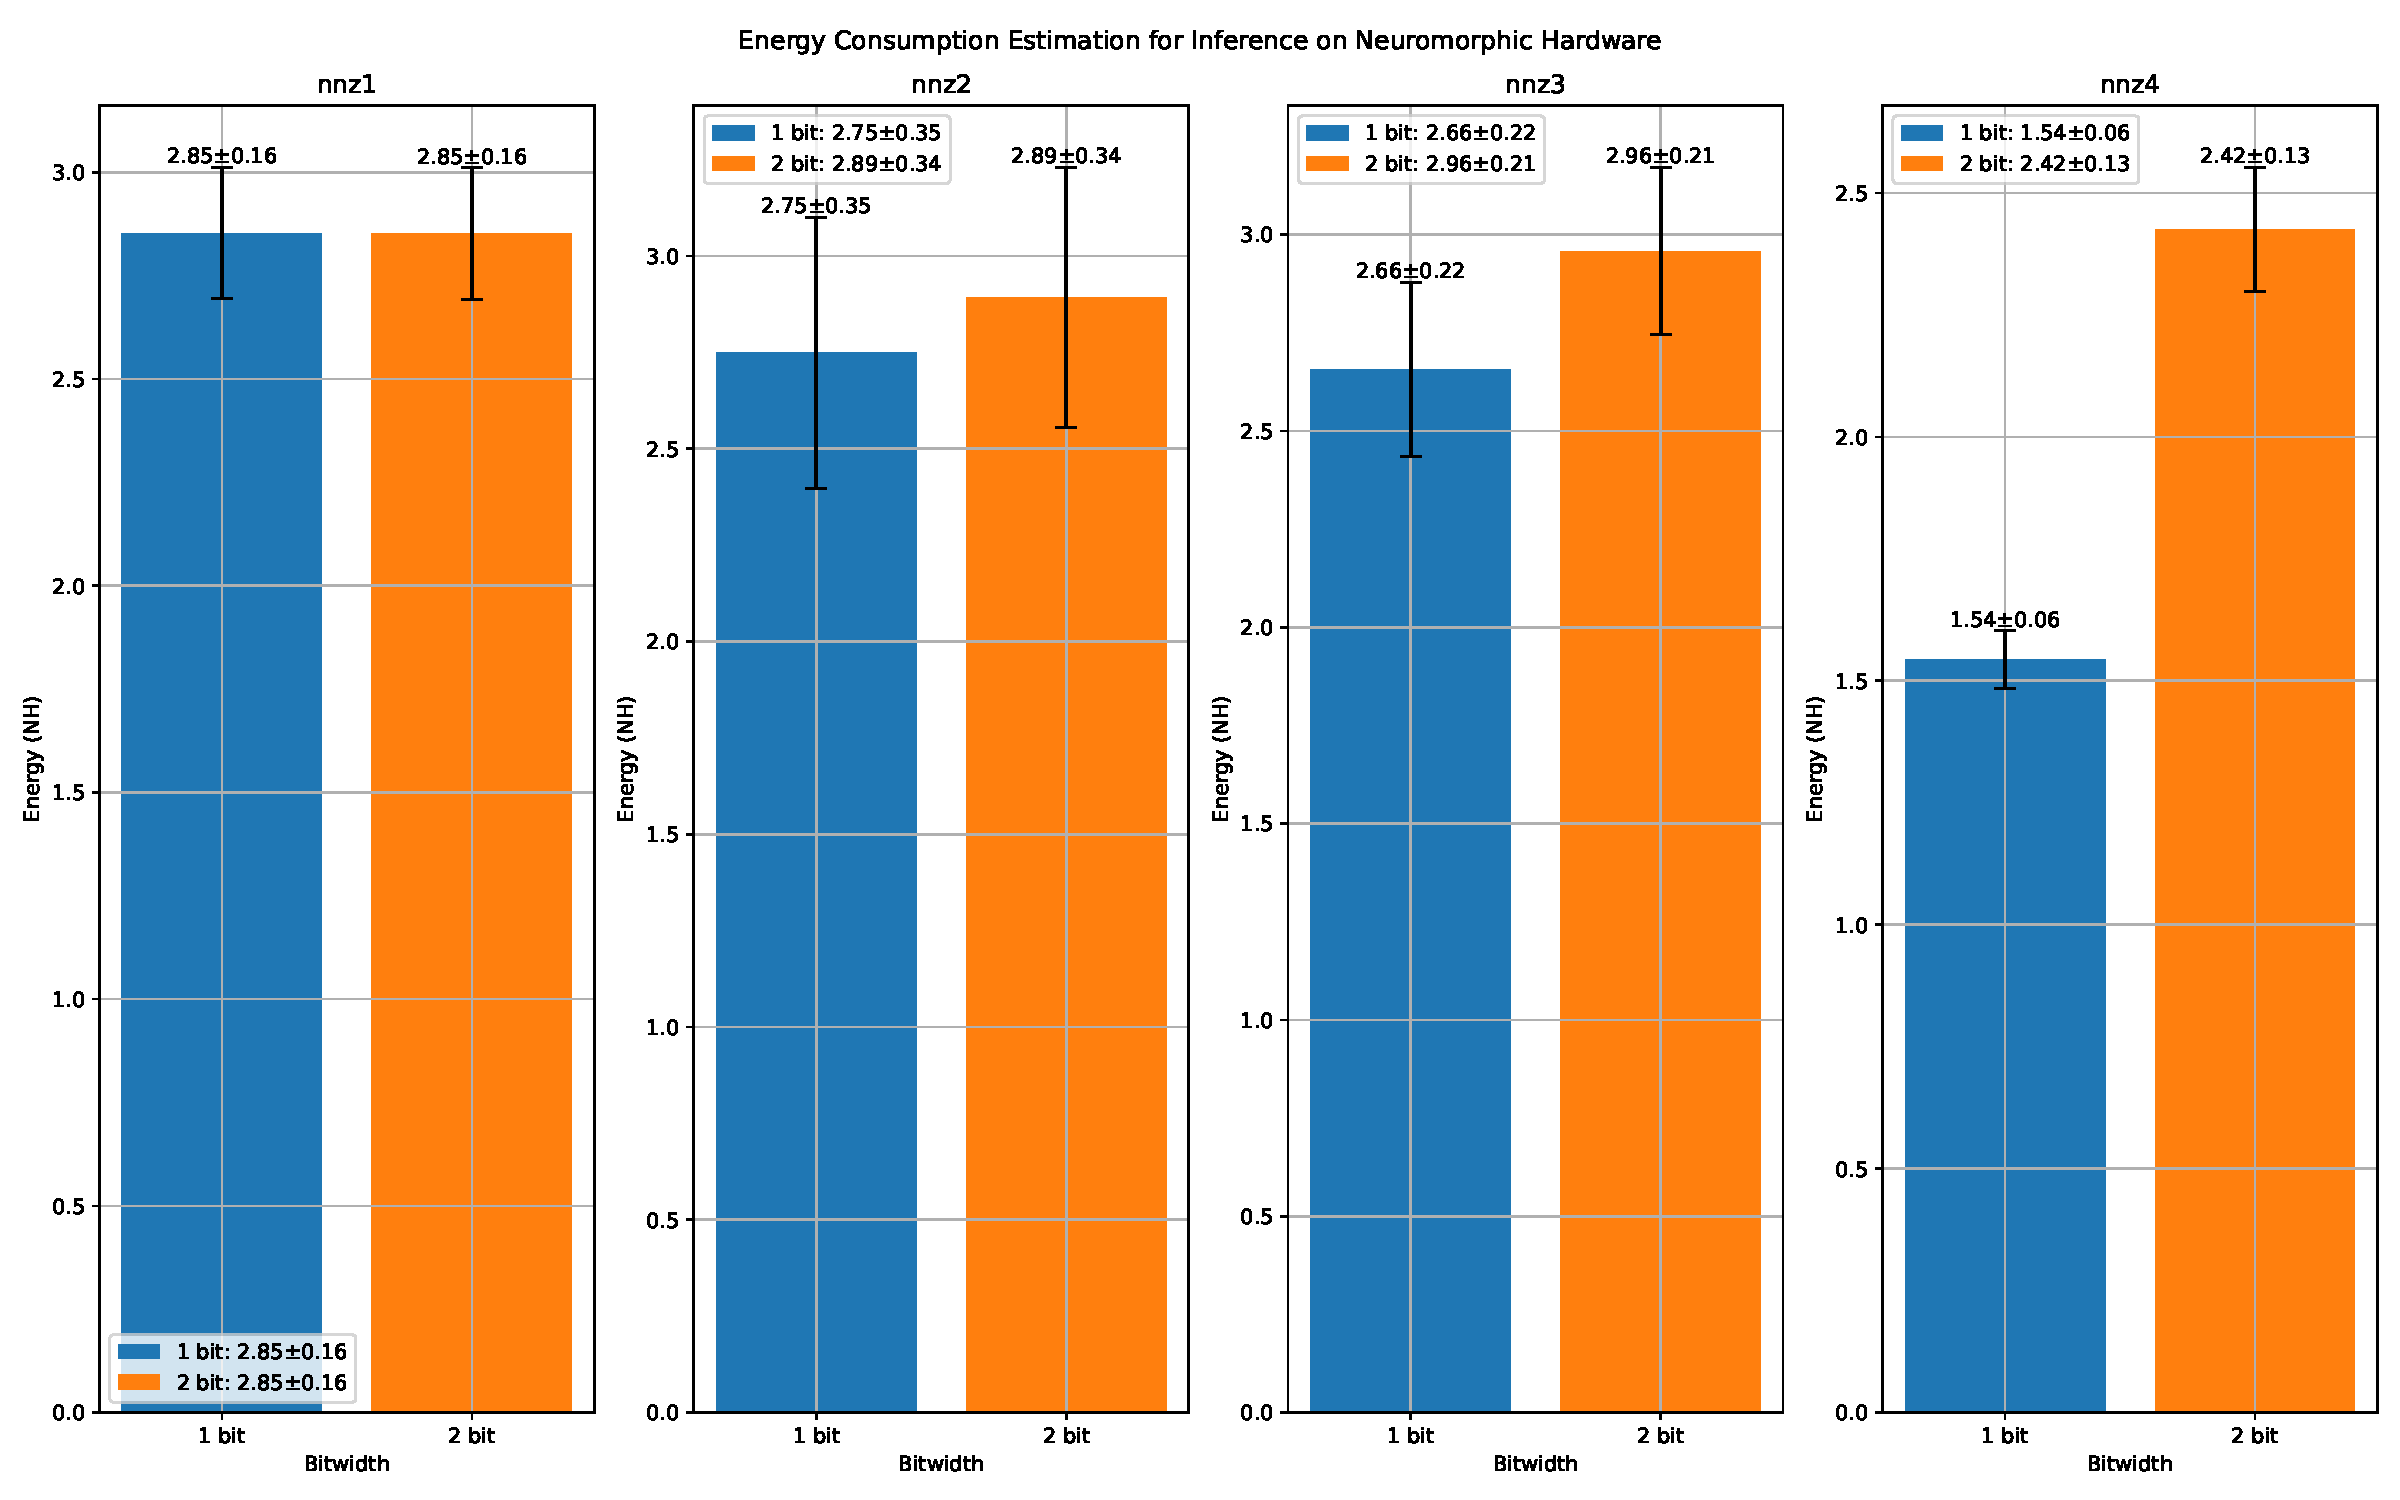
\includegraphics[width=\textwidth]{../firerate/FashionMNIST/plots/fashionmnist_test_energy_nh.pdf}
                \caption{Energy Consumption Estimation, Unit in Parameters $F\cdot E_{\text{AC}}$}
            \end{subfigure}
            \hfill
            \begin{subfigure}[H]{0.48\textwidth}
                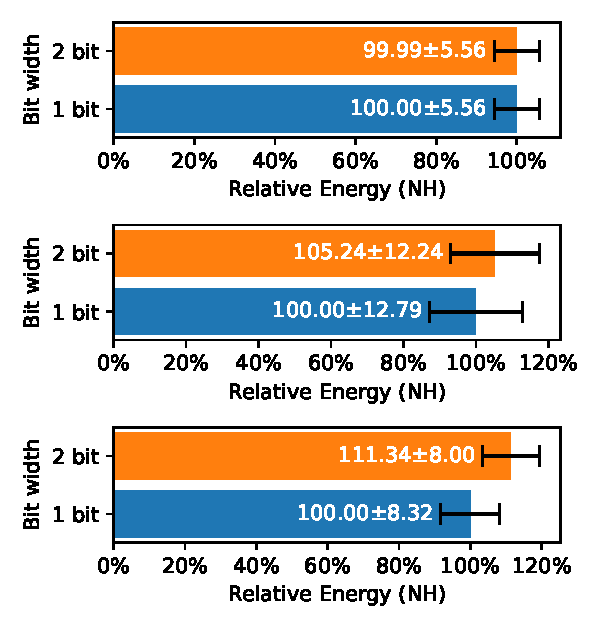
\includegraphics[width=\textwidth]{../firerate/FashionMNIST/plots/fashionmnist_test_relative_energy_nh.pdf}
                \caption{Normalized Energy Consumption Estimation Relative to 1-bit Spike Train Model}
            \end{subfigure}
            \caption{Inference Energy Consumption Estimation on Intel Loihi 2 for Fashion MNIST Dataset with 50 Training Epochs}
            \label{fig:inference_energy_nh_firerate}
        \end{figure}

        Additionally, if one is satisfied with the accuracy of the 1-bit spike train model, then one can choose to train the multi-bit spike train model for fewer time steps. This can enable higher efficiency in both training and inference. 

        We take again the example of the Fashion MNIST dataset, and while $T=10$ is a good choice for both the 1-bit and 2-bit spike train model, we can reduce the time steps to $T=4$ for the 2-bit spike train model and still achieve a comparable accuracy (see \ref{fig:inference_energy_nh_timesteps}). 
        \begin{figure}[!htpb]
            \centering
            \begin{subfigure}[H]{\textwidth}
                \centering
                \begin{subfigure}[H]{0.49\textwidth}
                    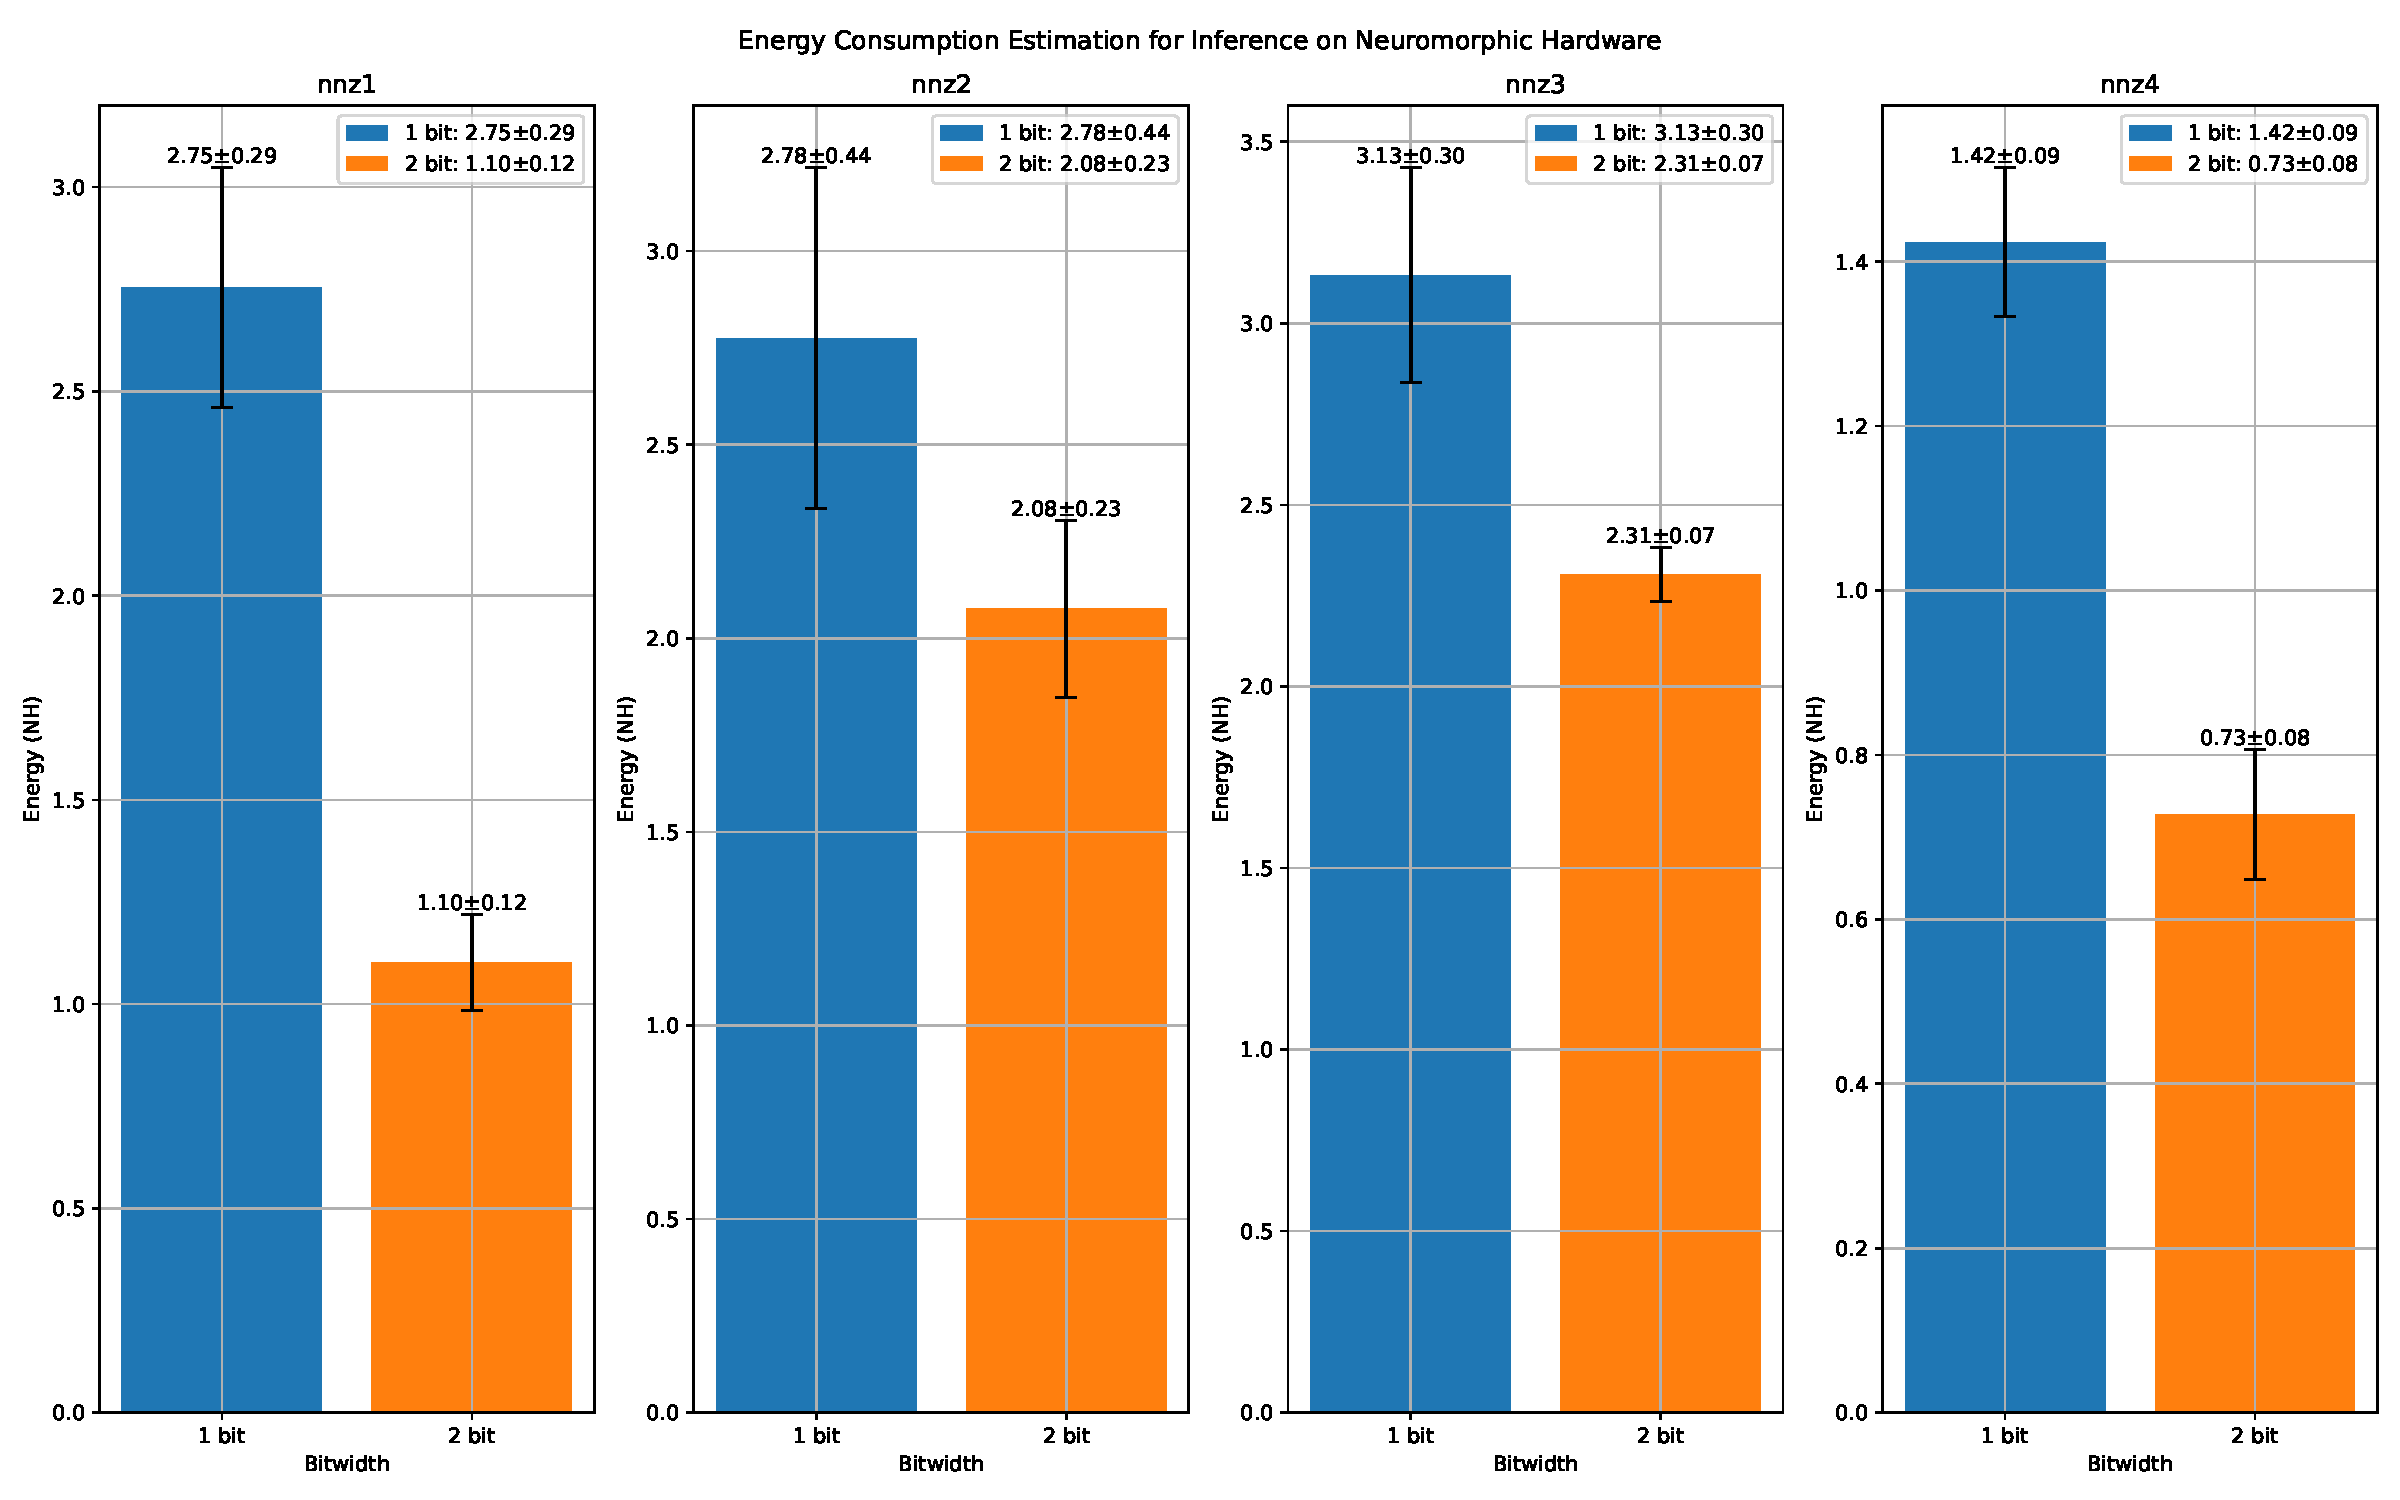
\includegraphics[width=\textwidth]{../timesteps/FashionMNIST/plots/fashionmnist_test_energy_nh.pdf}
                    \caption{Energy Consumption Estimation, Unit in Parameters $F\cdot E_{\text{AC}}$}
                \end{subfigure}
                \hfill
                \begin{subfigure}[H]{0.49\textwidth}
                    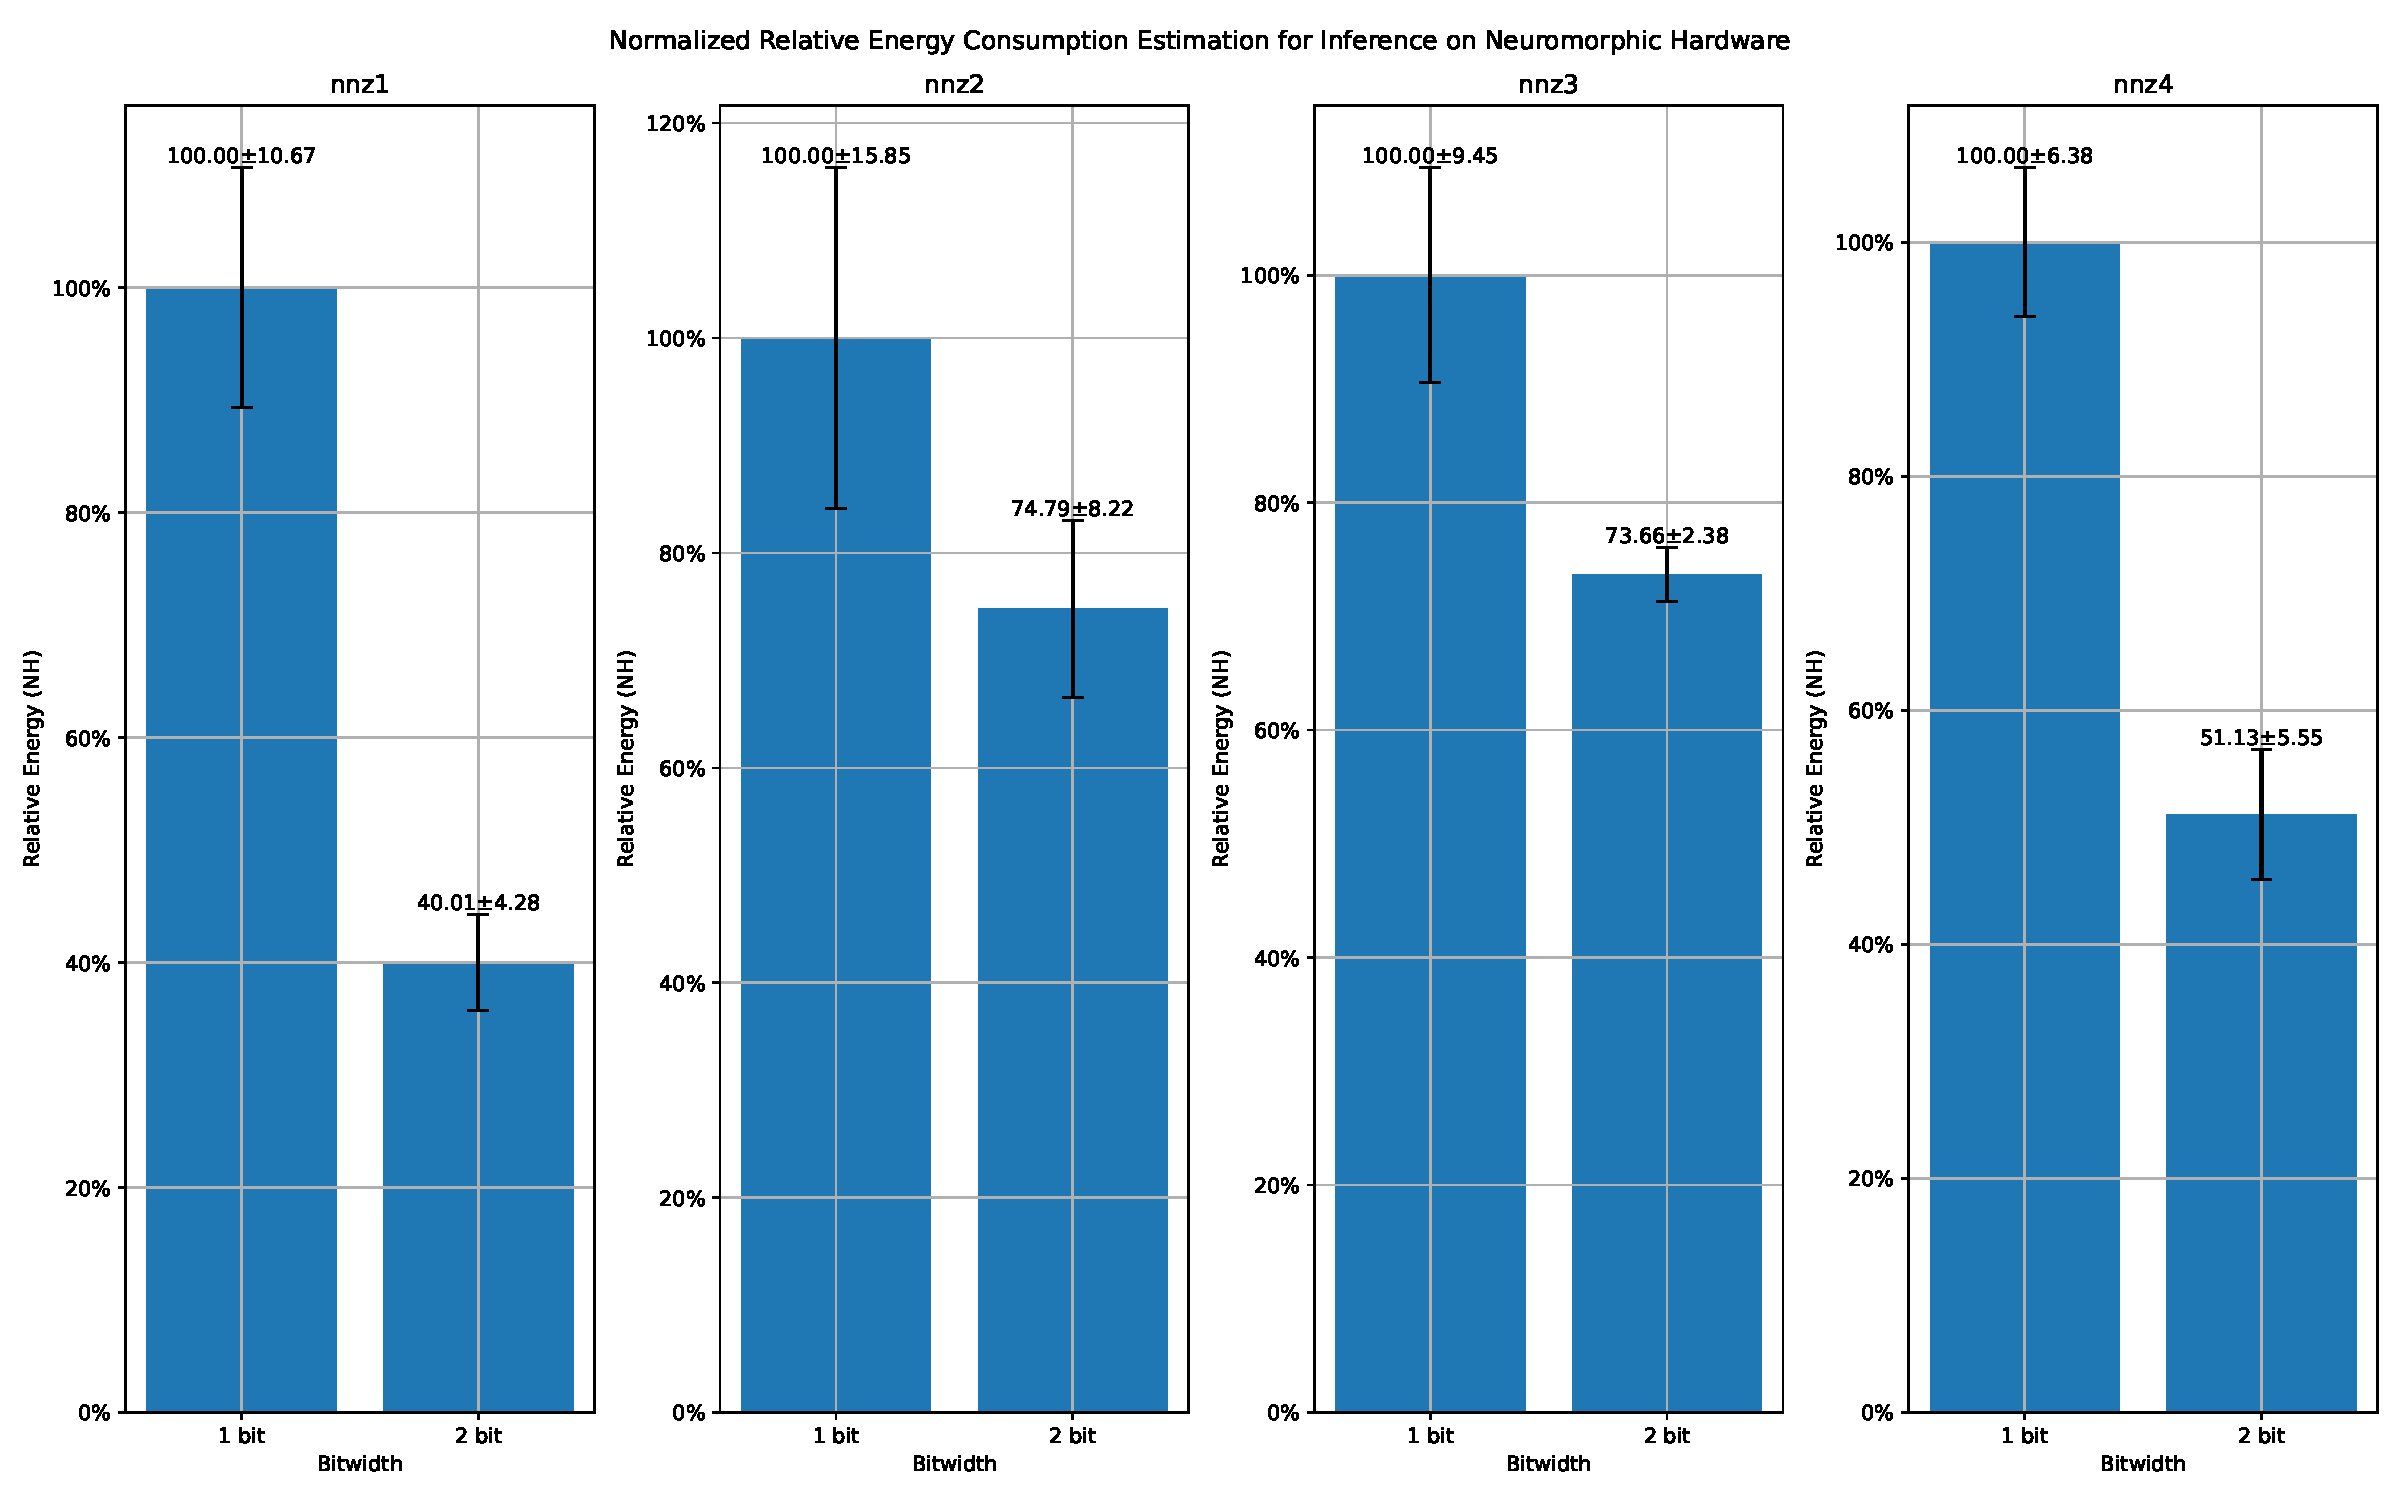
\includegraphics[width=\textwidth]{../timesteps/FashionMNIST/plots/fashionmnist_test_relative_energy_nh.pdf}
                    \caption{Normalized Energy Consumption Estimation Relative to 1-bit Spike Train Model}
                \end{subfigure}
            \end{subfigure}
            \hfill
            \begin{subfigure}[H]{\textwidth}
                \centering
                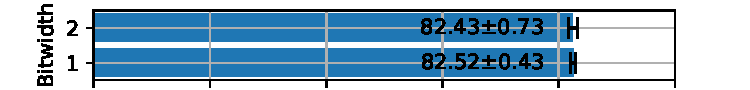
\includegraphics[width=\textwidth]{../timesteps/FashionMNIST/plots/fashionmnist_final_acc_horizontal.pdf}
                \caption{Accuracy Comparison}
            \end{subfigure}
            \caption{Inference Energy Consumption Estimation on Intel Loihi 2 and Test Accuracy for Fashion MNIST Dataset with 10 Time Steps for 1-bit Spike Train Model and 4 Time Steps for 2-bit Spike Train Model}
            \label{fig:inference_energy_nh_timesteps}
        \end{figure}
        
        More details with additional results on the CIFAR10 dataset can be found in Appendix \ref{appendix:energy_tradeoff}.

        The same tradeoffs allow the multi-bit spike train model to be more energy efficient than the ANN also for the Fashion MNIST dataset (see Figure \ref{fig:energy_ann_vs_snn_timesteps}).
        \begin{figure}[H]
            \centering
            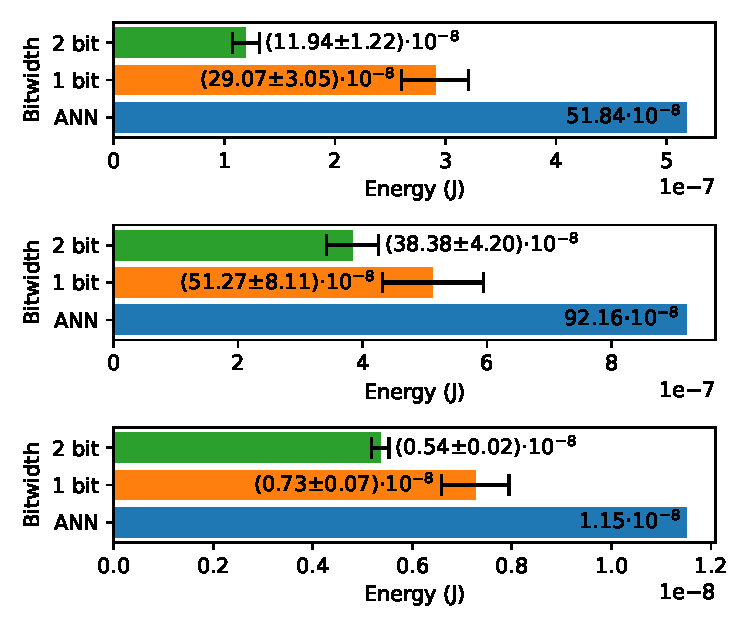
\includegraphics[width=0.6\textwidth]{../timesteps/FashionMNIST/plots/fashionmnist_energy_ann_vs_snn.pdf}
            \caption{Comparison of the Energy Consumption of ANN and Multi-Bit Spike Train Model on Intel Loihi 2 for Fashion MNIST Dataset with 10 Time Steps for 1-bit Spike Train Model and 4 Time Steps for 2-bit Spike Train Model, from top to bottom: first convolution block, second convolution block, output layer}
            \label{fig:energy_ann_vs_snn_timesteps}
        \end{figure}

        This can lead to a significant reduction in the energy consumption. It may not be reflected as a direct advantage in the energy consumption model mentioned above \ref{subsec:inference_energy}, but in practice, it should bring significant benefits, as most of the neuromorphic chips are designed to utilize the asynchronous communication via spikes, so they do not have a central clock system to synchronize the time steps very efficiently, and the cost for the synchronization barrier is very high. As reference, the latency per tile hop on Intel Loihi is at most around 6.5 ns where as the latency for the synchronization barrier is between 113 to 465 ns. 

\section{Performance}
\label{sec:performance}
    In the section \ref{subsec:training_energy}, we claim that the energy consumption on the GPUs are not affected by the firing rate and the bit width of the spike train in theory. However, in practice, with the increase of the bit width of the spike train, the training process slows down. This could be caused by the inefficient implementation of the multi-bit spike train model and the low level optimization on operations of sparse matrix multiplication. 

    There is sufficient room for improvement, e.g. by utilizing the sparsity of the spike trains or completely switching to the vectorized model instead of the temporal model instead, which is shown to be more efficient with learning algorithms like SLAYER and EXODUS. 
